%% abtex2-modelo-trabalho-academico.tex, v-1.9.2 laurocesar
%% Copyright 2012-2014 by abnTeX2 group at http://abntex2.googlecode.com/ 
%%
%% This work may be distributed and/or modified under the
%% conditions of the LaTeX Project Public License, either version 1.3
%% of this license or (at your option) any later version.
%% The latest version of this license is in
%%   http://www.latex-project.org/lppl.txt
%% and version 1.3 or later is part of all distributions of LaTeX
%% version 2005/12/01 or later.
%%
%% This work has the LPPL maintenance status `maintained'.
%% 
%% The Current Maintainer of this work is the abnTeX2 team, led
%% by Lauro César Araujo. Further information are available on 
%% http://abntex2.googlecode.com/
%%
%% This work consists of the files abntex2-modelo-trabalho-academico.tex,
%% abntex2-modelo-include-comandos and abntex2-modelo-references.bib
%%

% ------------------------------------------------------------------------
% ------------------------------------------------------------------------
% abnTeX2: Modelo de Trabalho Academico (tese de doutorado, dissertacao de
% mestrado e trabalhos monograficos em geral) em conformidade com 
% ABNT NBR 14724:2011: Informacao e documentacao - Trabalhos academicos -
% Apresentacao
% ------------------------------------------------------------------------
% ------------------------------------------------------------------------

%-------------------------------------------------------------------------
% Modelo adaptado especificamente para o contexto do PPgSI-EACH-USP por 
% Marcelo Fantinato, com auxílio dos Professores Norton T. Roman, Helton
% H. Bíscaro e Sarajane M. Peres, em 2015, com muitos agradecimentos aos 
% criadores da classe e do modelo base.
%
% 20/06/2017: inclusão de "lista de quadros" com base no especificado em:
% https://github.com/abntex/abntex2/wiki/HowToCriarNovoAmbienteListing,
% de autoria de "Eduardo de Santana Medeiros Alexandre".
%
%-------------------------------------------------------------------------

\documentclass[
	% -- opções da classe memoir --
	12pt,				% tamanho da fonte
	% openright,			% capítulos começam em pág ímpar (insere página vazia caso preciso)
	oneside,			% para impressão apenas no anverso (apenas frente). Oposto a twoside
	a4paper,			% tamanho do papel. 
	% -- opções da classe abntex2 --
	%chapter=TITLE,		% títulos de capítulos convertidos em letras maiúsculas
	%section=TITLE,		% títulos de seções convertidos em letras maiúsculas
	%subsection=TITLE,	% títulos de subseções convertidos em letras maiúsculas
	%subsubsection=TITLE,% títulos de subsubseções convertidos em letras maiúsculas
	% -- opções do pacote babel --
	english,			% idioma adicional para hifenização
	%french,				% idioma adicional para hifenização
	%spanish,			% idioma adicional para hifenização
	brazil				% o último idioma é o principal do documento
	]{abntex2ppgsi}

% ---
% Pacotes básicos 
% ---
% \usepackage{lmodern}			% Usa a fonte Latin Modern			
% \usepackage[T1]{fontenc}		% Selecao de codigos de fonte.
\usepackage[utf8]{inputenc}		% Codificacao do documento (conversão automática dos acentos)
\usepackage{lastpage}			% Usado pela Ficha catalográfica
\usepackage{indentfirst}		% Indenta o primeiro parágrafo de cada seção.
\usepackage{color}				% Controle das cores
\usepackage{graphicx}			% Inclusão de gráficos
\usepackage{microtype} 			% para melhorias de justificação
\usepackage{pdfpages}     %para incluir pdf
\usepackage{algorithm}			%para ilustrações do tipo algoritmo
\usepackage{mdwlist}			%para itens com espaço padrão da abnt
\usepackage[noend]{algpseudocode}			%para ilustrações do tipo algoritmo
		
% ---
% Pacotes adicionais, usados apenas no âmbito do Modelo Canônico do abnteX2
% ---
\usepackage{lipsum}				% para geração de dummy text
% ---

% ---
% Pacotes de citações
% ---
\usepackage[brazilian,hyperpageref]{backref}	 % Paginas com as citações na bibl
\usepackage[alf,abnt-etal-list=0,abnt-etal-text=it]{abntex2cite}	% Citações padrão ABNT

% --- 
% CONFIGURAÇÕES DE PACOTES
% --- 

% ---
% Configurações do pacote backref
% Usado sem a opção hyperpageref de backref
\renewcommand{\backrefpagesname}{Citado na(s) página(s):~}
% Texto padrão antes do número das páginas
\renewcommand{\backref}{}
% Define os textos da citação
\renewcommand*{\backrefalt}[4]{
	\ifcase #1 %
		Nenhuma citação no texto.%
	\or
		Citado na página #2.%
	\else
		Citado #1 vezes nas páginas #2.%
	\fi}%
% ---

% ---
% Informações de dados para CAPA e FOLHA DE ROSTO
% ---

%-------------------------------------------------------------------------
% Comentário adicional do PPgSI - Informações sobre o ``instituicao'':
%
% Não mexer. Deixar exatamente como está.
%
%-------------------------------------------------------------------------
\instituicao{
	UNIVERSIDADE DE SÃO PAULO
	\par
	ESCOLA DE ARTES, CIÊNCIAS E HUMANIDADES
	\par
	PROGRAMA DE PÓS-GRADUAÇÃO EM SISTEMAS DE INFORMAÇÃO}

%-------------------------------------------------------------------------
% Comentário adicional do PPgSI - Informações sobre o ``título'':
%
% Em maiúscula apenas a primeira letra da sentença (do título), exceto 
% nomes próprios, geográficos, institucionais ou Programas ou Projetos ou 
% siglas, os quais podem ter letras em maiúscula também.
%
% O subtítulo do trabalho é opcional.
% Sem ponto final.
%
% Atenção: o título da Dissertação na versão corrigida não pode mudar. 
% Ele deve ser idêntico ao da versão original.
%
%-------------------------------------------------------------------------
\titulo{Seleção entre estratégias de geração automática de dados de teste por meio de métricas estáticas de softwares orientados a objetos}

%-------------------------------------------------------------------------
% Comentário adicional do PPgSI - Informações sobre o ``autor'':
%
% Todas as letras em maiúsculas.
% Nome completo.
% Sem ponto final.
%-------------------------------------------------------------------------
\autor{\uppercase{GUSTAVO DA MOTA RAMOS}}

%-------------------------------------------------------------------------
% Comentário adicional do PPgSI - Informações sobre o ``local'':
%
% Não incluir o ``estado''.
% Sem ponto final.
%-------------------------------------------------------------------------
\local{São Paulo}

%-------------------------------------------------------------------------
% Comentário adicional do PPgSI - Informações sobre a ``data'':
%
% Colocar o ano do depósito (ou seja, o ano da entrega) da respectiva 
% versão, seja ela a versão original (para a defesa) seja ela a versão 
% corrigida (depois da aprovação na defesa). 
%
% Atenção: Se a versão original for depositada no final do ano e a versão 
% corrigida for entregue no ano seguinte, o ano precisa ser atualizado no 
% caso da versão corrigida. 
% Cuidado, pois o ano da ``capa externa'' também precisa ser atualizado 
% nesse caso.
%
% Não incluir o dia, nem o mês.
% Sem ponto final.
%-------------------------------------------------------------------------
\data{2018}

%-------------------------------------------------------------------------
% Comentário adicional do PPgSI - Informações sobre o ``Orientador'':
%
% Se for uma professora, trocar por ``Profa. Dra.''
% Nome completo.
% Sem ponto final.
%-------------------------------------------------------------------------
\orientador{Prof. Dr. Marcelo Medeiros Eler}

%-------------------------------------------------------------------------
% Comentário adicional do PPgSI - Informações sobre o ``Coorientador'':
%
% Opcional. Incluir apenas se houver co-orientador formal, de acordo com o 
% Regulamento do Programa.
%
% Se for uma professora, trocar por ``Profa. Dra.''
% Nome completo.
% Sem ponto final.
%-------------------------------------------------------------------------
%\coorientador{Prof. Dr. Fulano de Tal}

\tipotrabalho{Dissertação (Mestrado)}

\preambulo{
%-------------------------------------------------------------------------
% Comentário adicional do PPgSI - Informações sobre o texto ``Versão 
% original'':
%
% Não usar para Qualificação.
% Não usar para versão corrigida de Dissertação.
%
%-------------------------------------------------------------------------
Versão original \newline \newline \newline 
%-------------------------------------------------------------------------
% Comentário adicional do PPgSI - Informações sobre o ``texto principal do
% preambulo'':
%
% Para Qualificação, trocar por: Texto de Exame de Qualificação apresentado à Escola de Artes, Ciências e Humanidades da Universidade de São Paulo como parte dos requisitos para obtenção do título de Mestre em Ciências pelo Programa de Pós-graduação em Sistemas de Informação.
%
%-------------------------------------------------------------------------
Dissertação apresentada à Escola de Artes, Ciências e Humanidades da Universidade de São Paulo para obtenção do título de Mestre em Ciências pelo Programa de Pós-graduação em Sistemas de Informação. 
%
\newline \newline Área de concentração: Metodologia e Técnicas da Computação
%-------------------------------------------------------------------------
% Comentário adicional do PPgSI - Informações sobre o texto da ``Versão 
% corrigida'':
%
% Não usar para Qualificação.
% Não usar para versão original de Dissertação.
% 
% Substituir ``xx de xxxxxxxxxxxxxxx de xxxx'' pela ``data da defesa''.
%
%-------------------------------------------------------------------------
\newline \newline \newline }
% ---


% ---
% Configurações de aparência do PDF final

% alterando o aspecto da cor azul
\definecolor{blue}{RGB}{41,5,195}

% informações do PDF
\makeatletter
\hypersetup{
     	%pagebackref=true,
		pdftitle={\@title}, 
		pdfauthor={\@author},
    	pdfsubject={\imprimirpreambulo},
	    pdfcreator={LaTeX com abnTeX2 adaptado para o PPgSI-EACH-USP},
		pdfkeywords={abnt}{latex}{abntex}{abntex2}{qualificação de mestrado}{dissertação de mestrado}{ppgsi}, 
		colorlinks=true,       		% false: boxed links; true: colored links
    	linkcolor=black,          	% color of internal links
    	citecolor=black,        		% color of links to bibliography
    	filecolor=black,      		% color of file links
		urlcolor=black,
		bookmarksdepth=4
}
\makeatother
% --- 

% --- 
% Espaçamentos entre linhas e parágrafos 
% --- 

% O tamanho do parágrafo é dado por:
\setlength{\parindent}{1.25cm}

% Controle do espaçamento entre um parágrafo e outro:
\setlength{\parskip}{0cm}  % tente também \onelineskip
\renewcommand{\baselinestretch}{1.5}

% ---
% compila o indice
% ---
\makeindex
% ---

	% Controlar linhas orfas e viuvas
  \clubpenalty10000
  \widowpenalty10000
  \displaywidowpenalty10000

% ----
% Início do documento
% ----
\begin{document}

% Retira espaço extra obsoleto entre as frases.
\frenchspacing 

% ----------------------------------------------------------
% ELEMENTOS PRÉ-TEXTUAIS
% ----------------------------------------------------------
% \pretextual

% ---
% Capa
% ---
%-------------------------------------------------------------------------
% Comentário adicional do PPgSI - Informações sobre a ``capa'':
%
% Esta é a ``capa'' principal/oficial do trabalho, a ser impressa apenas 
% para os casos de encadernação simples (ou seja, em ``espiral'' com 
% plástico na frente).
% 
% Não imprimir esta ``capa'' quando houver ``capa dura'' ou ``capa brochura'' 
% em que estas mesmas informações já estão presentes nela.
%
%-------------------------------------------------------------------------
\imprimircapa
% ---

% ---
% Folha de rosto
% (o * indica que haverá a ficha bibliográfica)
% ---
\imprimirfolhaderosto*
% ---

% ---
% Inserir a autorização para reprodução e ficha bibliografica
% ---

%-------------------------------------------------------------------------
% Comentário adicional do PPgSI - Informações sobre o texto da 
% ``autorização para reprodução e ficha bibliografica'':
%
% Página a ser usada apenas para Dissertação (tanto na versão original 
% quanto na versão corrigida).
%
% Solicitar a ficha catalográfica na Biblioteca da EACH. 
% Duas versões devem ser solicitadas, em dois momentos distintos: uma vez 
% para a versão original, e depois outra atualizada para a versão 
% corrigida.
%
% Atenção: esta página de ``autorização para reprodução e ficha 
% catalográfica'' deve ser impressa obrigatoriamente no verso da folha de 
% rosto.
%
% Não usar esta página para Qualificação.
%
% Substitua o arquivo ``fig_ficha_catalografica.pdf'' abaixo referenciado 
% pelo PDF elaborado pela Biblioteca
%
%-------------------------------------------------------------------------
\begin{fichacatalografica}
    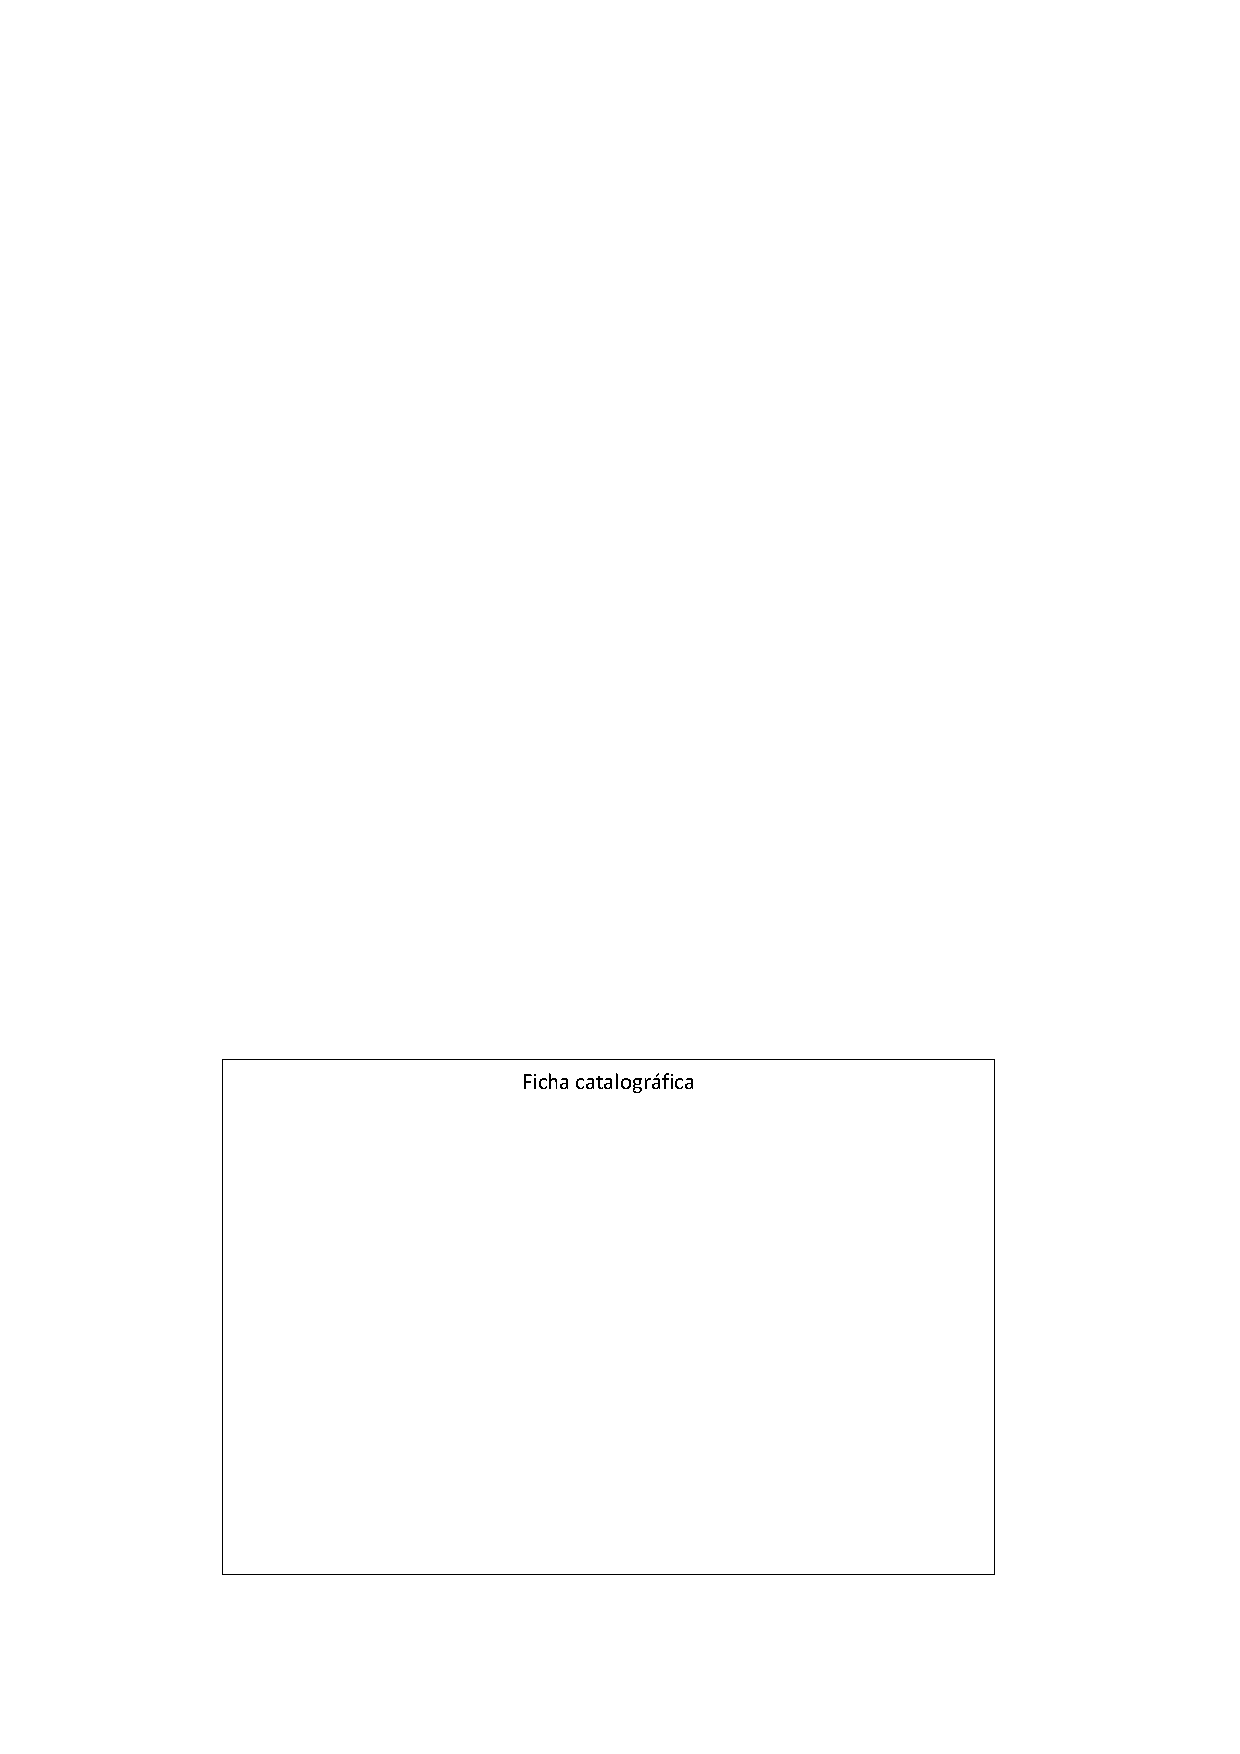
\includepdf{fig_ficha_catalografica.pdf}
\end{fichacatalografica}

% ---
% Inserir errata
% ---
%-------------------------------------------------------------------------
% Comentário adicional do PPgSI - Informações sobre ``Errata'':
%
% Usar esta página de errata apenas em casos de excepcionais, e apenas 
% para a versão corrigida da Dissertação. Por exemplo, quando depois de
% já depositada e publicada a versão corrigida, ainda assim verifica-se
% a necessidade de alguma correção adicional.
%
% Se precisar usar esta página, busque a forma correta (o modelo correto) 
% para fazê-lo, de acordo com a norma ABNT.
%
% Não usar esta página para versão original de Dissertação.
% Não usar esta página para Qualificação.
%
%-------------------------------------------------------------------------
%\begin{errata}
%Elemento opcional para versão corrigida, depois de depositada.
%\end{errata}
% ---

% ---
% Inserir folha de aprovação
% ---

\begin{folhadeaprovacao}
%-------------------------------------------------------------------------
% Comentário adicional do PPgSI - Informações sobre ``Folha da aprovação'':
%
% Página a ser usada apenas para Dissertação.
%
% Não usar esta página para Qualificação.
%
% Substituir ``Fulano de Tal'' pelo nome completo do autor do trabalho, com 
% apenas as iniciais em maiúsculo.
%
% Substituir ``___ de ______________ de ______'' por: 
%     - Para versão original de Dissertação: deixar em branco, pois a data 
%       pode mudar, mesmo que ela já esteja prevista.
%     - Para versão corrigida de Dissertação: usar a data em que a defesa 
%       efetivamente ocorreu.
%
%-------------------------------------------------------------------------
\noindent Dissertação de autoria de Gustavo da Mota Ramos, sob o título \textbf{``\imprimirtitulo''}, apresentada à Escola de Artes, Ciências e Humanidades da Universidade de São Paulo, para obtenção do título de Mestre em Ciências pelo Programa de Pós-graduação em Sistemas de Informação, na área de concentração Metodologia e Técnicas da Computação, aprovada em \_\_\_\_\_\_\_ de \_\_\_\_\_\_\_\_\_\_\_\_\_\_\_\_\_\_\_\_\_\_ de \_\_\_\_\_\_\_\_\_\_ pela comissão julgadora constituída pelos doutores:

\vspace*{3cm}

\begin{center}
%-------------------------------------------------------------------------
% Comentário adicional do PPgSI - Informações sobre ``assinaturas'':
%
% Para versão original de Dissertação: deixar em 
% branco (ou seja, assim como está abaixo), pois os membros da banca podem
% mudar, mesmo que eles já estejam previstos.
% 
% Para versão corrigida de Dissertação: usar os dados dos examinadores que 
% efetivamente participaram da defesa. 
% 
% Para versão corrigida de Dissertação: em caso de ``professora'', trocar 
% por ``Profa. Dra.'' 
% 
% Para versão corrigida de Dissertação: ao colocar os nomes dos 
% examinadores, remover o sublinhado
% 
% Para versão corrigida de Dissertação: ao colocar os nomes dos 
% examinadores, usar seus nomes completos, exatamente conforme constam em 
% seus Currículos Lattes
% 
% Para versão corrigida de Dissertação: ao colocar os nomes das 
% instituições, remover o sublinhado e remover a palavra ``Instituição:''
%
% Não abreviar os nomes das instituições.
%
%-------------------------------------------------------------------------
\_\_\_\_\_\_\_\_\_\_\_\_\_\_\_\_\_\_\_\_\_\_\_\_\_\_\_\_\_\_\_\_\_\_\_\_\_\_\_\_\_\_\_\_\_\_\_\_\_\_\_\_\_\_\_\_
\vspace*{0.2cm} 
\\ \textbf{Prof. Dr. \_\_\_\_\_\_\_\_\_\_\_\_\_\_\_\_\_\_\_\_\_\_\_\_\_\_\_\_\_\_\_\_\_\_\_\_\_\_\_\_\_\_\_\_\_\_\_\_\_\_\_\_\_\_\_\_\_\_\_\_\_\_} 
\\ \vspace*{0.2cm} 
Instituição: \_\_\_\_\_\_\_\_\_\_\_\_\_\_\_\_\_\_\_\_\_\_\_\_\_\_\_\_\_\_\_\_\_\_\_\_\_\_\_\_\_\_\_\_\_\_\_\_\_\_\_\_\_\_\_\_\_\_ 
\\ \vspace*{0.2cm}
Presidente 

\vspace*{2cm}

\_\_\_\_\_\_\_\_\_\_\_\_\_\_\_\_\_\_\_\_\_\_\_\_\_\_\_\_\_\_\_\_\_\_\_\_\_\_\_\_\_\_\_\_\_\_\_\_\_\_\_\_\_\_\_\_
\vspace*{0.2cm} 
\\ \textbf{Prof. Dr. \_\_\_\_\_\_\_\_\_\_\_\_\_\_\_\_\_\_\_\_\_\_\_\_\_\_\_\_\_\_\_\_\_\_\_\_\_\_\_\_\_\_\_\_\_\_\_\_\_\_\_\_\_\_\_\_\_\_\_\_\_\_} 
\\ \vspace*{0.2cm} 
Instituição: \_\_\_\_\_\_\_\_\_\_\_\_\_\_\_\_\_\_\_\_\_\_\_\_\_\_\_\_\_\_\_\_\_\_\_\_\_\_\_\_\_\_\_\_\_\_\_\_\_\_\_\_\_\_\_\_\_\_

\vspace*{2cm}

\_\_\_\_\_\_\_\_\_\_\_\_\_\_\_\_\_\_\_\_\_\_\_\_\_\_\_\_\_\_\_\_\_\_\_\_\_\_\_\_\_\_\_\_\_\_\_\_\_\_\_\_\_\_\_\_
\vspace*{0.2cm} 
\\ \textbf{Prof. Dr. \_\_\_\_\_\_\_\_\_\_\_\_\_\_\_\_\_\_\_\_\_\_\_\_\_\_\_\_\_\_\_\_\_\_\_\_\_\_\_\_\_\_\_\_\_\_\_\_\_\_\_\_\_\_\_\_\_\_\_\_\_\_} 
\\ \vspace*{0.2cm} 
Instituição: \_\_\_\_\_\_\_\_\_\_\_\_\_\_\_\_\_\_\_\_\_\_\_\_\_\_\_\_\_\_\_\_\_\_\_\_\_\_\_\_\_\_\_\_\_\_\_\_\_\_\_\_\_\_\_\_\_\_

\vspace*{2cm}

\_\_\_\_\_\_\_\_\_\_\_\_\_\_\_\_\_\_\_\_\_\_\_\_\_\_\_\_\_\_\_\_\_\_\_\_\_\_\_\_\_\_\_\_\_\_\_\_\_\_\_\_\_\_\_\_
\vspace*{0.2cm} 
\\ \textbf{Prof. Dr. \_\_\_\_\_\_\_\_\_\_\_\_\_\_\_\_\_\_\_\_\_\_\_\_\_\_\_\_\_\_\_\_\_\_\_\_\_\_\_\_\_\_\_\_\_\_\_\_\_\_\_\_\_\_\_\_\_\_\_\_\_\_} 
\\ \vspace*{0.2cm} 
Instituição: \_\_\_\_\_\_\_\_\_\_\_\_\_\_\_\_\_\_\_\_\_\_\_\_\_\_\_\_\_\_\_\_\_\_\_\_\_\_\_\_\_\_\_\_\_\_\_\_\_\_\_\_\_\_\_\_\_\_

\end{center}
  
\end{folhadeaprovacao}
% ---

% ---
% Dedicatória
% ---
%-------------------------------------------------------------------------
% Comentário adicional do PPgSI - Informações sobre ``Dedicatória'': 
%
% Opcional para Dissertação.
% Não sugerido para Qualificação.
% 
%-------------------------------------------------------------------------
\begin{dedicatoria}
   \vspace*{\fill}
   \centering
   \noindent
   \textit{Aos meus pais, Nivaldo e Izildinha, que não mediram esforços para que eu chegasse até aqui. Eles são responsáveis pela maior herança da minha vida: meus estudos.} 
	 \vspace*{\fill}
\end{dedicatoria}
% ---

% ---
% Agradecimentos
% ---
%-------------------------------------------------------------------------
% Comentário adicional do PPgSI - Informações sobre ``Agradecimentos'': 
%
% Opcional para Dissertação.
% Não sugerido para Qualificação.
% 
% Lembrar de agradecer agências de fomento e outras instituições similares.
%
%-------------------------------------------------------------------------

% ---

% ---
% Epígrafe
% ---
%-------------------------------------------------------------------------
% Comentário adicional do PPgSI - Informações sobre ``Epígrafe'': 
%
% Opcional para Dissertação.
% Não sugerido para Qualificação.
% 
%-------------------------------------------------------------------------

% ---

% ---
% RESUMOS
% ---

% resumo em português
\setlength{\absparsep}{18pt} % ajusta o espaçamento dos parágrafos do resumo
\begin{resumo}

%-------------------------------------------------------------------------
% Comentário adicional do PPgSI - Informações sobre ``referência'':
% 
% Troque os seguintes campos pelos dados de sua Dissertação (mantendo a 
% formatação e pontuação):
%   - SOBRENOME
%   - Nome1
%   - Nome2
%   - Nome3
%   - Título do trabalho: subtítulo do trabalho
%   - AnoDeDefesa
%
% Mantenha todas as demais informações exatamente como estão.
% 
% [Não usar essas informações de ``referência'' para Qualificação]
%
%-------------------------------------------------------------------------
\begin{flushleft}
RAMOS, Gustavo da Mota. \textbf{Título do trabalho}: Seleção entre estratégias de geração automática de dados de teste por meio de métricas estáticas de softwares orientados a objetos. \imprimirdata. 75p f. Dissertação (Mestrado em Ciências) – Escola de Artes, Ciências e Humanidades, Universidade de São Paulo, São Paulo, 2018.
\end{flushleft}

Produtos de software com diferentes complexidade são criados diariamente através da elicitação de demandas complexas e variadas juntamente a prazos restritos. Enquanto estes surgem, altos níveis de qualidade são esperados para tais, ou seja, enquanto os produtos tornam-se mais complexos, o nível de qualidade pode não ser aceitável enquanto o tempo hábil para testes não acompanha a complexidade. Desta maneira, o teste de software e a geração automática de dados de testes surgem com o intuito de entregar produtos contendo altos níveis de qualidade através de baixos custos e atividades rápidas de teste. Porém, neste contexto, os profissionais de desenvolvimento dependem das estratégias de geração automáticas de testes e principalmente da seleção da técnica mais adequada para conseguir maior cobertura de código possível, este é um fator importante dados que cada técnica de geração de dados de teste possuem particularidades e problemas que fazem seu uso melhor em determinados tipos de software. A partir desde cenário, o presente trabalho propõe a seleção da técnica adequada para cada classe de um software com base em suas características, expressas por meio de métricas de softwares orientados a objetos a partir do algoritmo de classificação naive bayes.
Inicialmente foi realizado uma revisão bilbiográfica dos dois algoritmos de geração estudos, algoritmo de busca randômico e algoritmo de busca genético, compreendendo assim suas vantagens e desvantagens tanto de implementação como de execução. As métricas CK também foram estudadas com o intuito de compreender como estas podem descrever melhor as características de uma classe. O conhecimento adquirido possibilitou coletar os dados de geração de testes de cada classe como cobertura de código e tempo de geração a partir de cada técnica e também as métricas CK, permitindo assim a análise destes dados em conjunto e por fim execução do algoritmo de classificação. Os resultados desta análise demonstraram que um conjunto reduzido e selecionado de métricas é mais eficiente e descreve melhor as características de uma classe além de demonstrarem que as métricas CK possuem pouca ou nenhuma influência no tempo de geração dos dados de teste e no algoritmo de busca randômico. Entretando, as métricas CK demonstraram média correlação e influência na seleção do algoritmo genético, participando assim na sua seleção pelo algoritmo naive bayes.


Palavras-chaves: Métricas CK. Teste de software. Geração de testes. Cobertura de testes. Naive bayes. Algoritmo genético. 
\end{resumo}

% resumo em inglês
%-------------------------------------------------------------------------
% Comentário adicional do PPgSI - Informações sobre ``resumo em inglês''
% 
% Caso a Qualificação ou a Dissertação inteira seja elaborada no idioma inglês, 
% então o ``Abstract'' vem antes do ``Resumo''.
% 
%-------------------------------------------------------------------------
\begin{resumo}[Abstract]
\begin{otherlanguage*}{english}

%-------------------------------------------------------------------------
% Comentário adicional do PPgSI - Informações sobre ``referência em inglês''
% 
% Troque os seguintes campos pelos dados de sua Dissertação (mantendo a 
% formatação e pontuação):
%     - SURNAME
%     - FirstName1
%     - MiddleName1
%     - MiddleName2
%     - Work title: work subtitle
%     - DefenseYear (Ano de Defesa)
%
% Mantenha todas as demais informações exatamente como estão.
%
% [Não usar essas informações de ``referência'' para Qualificação]
%
%-------------------------------------------------------------------------
\begin{flushleft}
RAMOS, Gustavo da Mota. \textbf{Work title}: Selection between whole test generation strategies by analysing object oriented software  static metrics .  \imprimirdata. 75 p. Dissertation (Master of Science) – School of Arts, Sciences and Humanities, University of São Paulo, São Paulo, DefenseYear. 
\end{flushleft}

Software products with different complexity are created daily through analysis of complex and varied demands together with tight deadlines. While these arise, high levels of quality are expected for such, as products become more complex, the quality level may not be acceptable while the timing for testing does not keep up with complexity. In this way, software testing and automatic generation of test data arise in order to deliver products containing high levels of quality through low cost and rapid test activities. However, in this context, software developers depend on the strategies of automatic generation of tests and especially on the selection of the most adequate technique to obtain greater code coverage possible, this is an important factor given that each technique of data generation of test have peculiarities and problems that make its use better in certain types of software. From this scenario, the present work proposes the selection of the appropriate technique for each class of software based on its characteristics, expressed through object oriented software metrics from the naive bayes classification algorithm.
Initially, a literature review of the two generation algorithms was carried out, random search algorithm and genetic search algorithm, thus understanding its advantages and disadvantages in both implementation and execution. The CK metrics have also been studied in order to understand how they can better describe the characteristics of a class. The acquired knowledge allowed to collect the generation data of tests of each class as code coverage and generation time from each technique and also the CK metrics, thus allowing the analysis of these data together and finally execution of the classification algorithm. The results of this analysis demonstrated that a reduced and selected set of metrics is more efficient and better describes the characteristics of a class besides demonstrating that the CK metrics have little or no influence on the generation time of the test data and on the random search algorithm . However, the CK metrics showed a medium correlation and influence in the selection of the genetic algorithm, thus participating in its selection by the algorithm naive bayes.

Keywords: CK metrics. Software testing. Test data generation. Code coverages. Naive bayes. Genetic algorithm.
\end{otherlanguage*}
\end{resumo}

% ---
% ---
% inserir lista de figuras
% ---
\pdfbookmark[0]{\listfigurename}{lof}
\listoffigures*
\cleardoublepage
% ---

% ---
% inserir lista de algoritmos
% ---
\pdfbookmark[0]{\listalgorithmname}{loa}
\listofalgorithms
\cleardoublepage

% ---
% inserir lista de quadros
% ---
\pdfbookmark[0]{\listofquadrosname}{loq}
\listofquadros*
\cleardoublepage


% ---
% inserir lista de tabelas
% ---
\pdfbookmark[0]{\listtablename}{lot}
\listoftables*
\cleardoublepage
% ---

% ---
% inserir lista de abreviaturas e siglas
% ---
%-------------------------------------------------------------------------
% Comentário adicional do PPgSI - Informações sobre ``Lista de abreviaturas 
% e siglas'': 
%
% Opcional.
% Uma vez que se deseja usar, é necessário manter padrão e consistência no
% trabalho inteiro.
% Se usar: inserir em ordem alfabética.
%
%-------------------------------------------------------------------------
\begin{siglas}
  \item[CBO] \textit{Coupling between objects}
\item[CK] \textit{Chidamber \& Kemerer}
 \item[CUT] \textit{Class under test}
 \item[DIT] \textit{Depth inheritance tree}
 \item[LCOM] \textit{Lack of cohesion of methods}
 \item[LOC] \textit{Lines of code}
 \item[NOC] \textit{Number of children}
 \item[NOF] \textit{Number of fields}
 \item[NOM] \textit{Number of methods}
 \item[NOPF] \textit{Number of public fields}
 \item[NOPM] \textit{Number of public methods}
 \item[RFC] \textit{Response for a Class}
  \item[SUT] \textit{Software under test}
   \item[WMC] \textit{Weight method class}
\end{siglas}
% ---

% ---
% inserir lista de símbolos
% ---
%-------------------------------------------------------------------------
% Comentário adicional do PPgSI - Informações sobre ``Lista de símbolos'': 
%
% Opcional.
% Uma vez que se deseja usar, é necessário manter padrão e consistência no
% trabalho inteiro.
% Se usar: inserir na ordem em que aparece no texto.
% 
%-------------------------------------------------------------------------

% ---

% ---
% inserir o sumario
% ---
\pdfbookmark[0]{\contentsname}{toc}
\tableofcontents*
\cleardoublepage
% ---



% ----------------------------------------------------------
% ELEMENTOS TEXTUAIS
% ----------------------------------------------------------
\textual



%-------------------------------------------------------------------------
% Comentário adicional do PPgSI - Informações sobre ``títulos de seções''
% 
% Para todos os títulos (seções, subseções, tabelas, ilustrações, etc.):
%
% Em maiúscula apenas a primeira letra da sentença (do título), exceto 
% nomes próprios, geográficos, institucionais ou Programas ou Projetos ou
% siglas, os quais podem ter letras em maiúscula também.
%
%-------------------------------------------------------------------------
\chapter{Introdução}
\label{chap:introducao}
Produtos de software de diferentes tamanhos e complexidades são utilizados todos os dias em atividades profissionais ou de entretenimento. Em qualquer circunstância, entretanto, a falta de qualidade em produtos pode caracterizar uma situação preocupante para seus produtores \cite{hilburn2002software}  \cite{binder1994test}, uma vez que cada vez mais os níveis aceitáveis de qualidade de um software estão aumentando, tanto no que se refere ao seu comportamento observável externamente quanto ao seu processo de desenvolvimento e estrutura interna \cite{linda2006quality} \cite{bashir2008test} \cite{graham2008foundations}.


O teste de software \cite{tahir2014test} é a maneira mais popular de verificar se um software atende às especificações descritas e cumpre o papel desejado pelos interessados \cite{sommerville2008engenharia}. Ela consiste na execução do programa sob teste para revelar seus defeitos. Para isso, casos de teste são gerados de maneira que satisfaçam a diversos critérios, em geral baseados na especificação e na implementação do software \cite{pezze2008software}. 

Entretanto, gerar casos de teste para testar o software nos mais diversos contextos e dados de entrada é uma das atividades mais custosas no ciclo de vida de software, requisitando muito tempo e esforço para o seu planejamento, execução e manutenção. \cite{tahir2014test}. Consequentemente, pesquisadores e profissionais da área passaram então a desenvolver  abordagens para gerar casos de teste automaticamente e assim reduzir o custo e a complexidade desta tarefa. Diversas técnicas já foram utilizadas com teste objetivo: geração de testes randômicos \cite{Pacheco2007}; execução simbólica \cite{Cadar2013}; teste baseado em modelos \cite{dick93}; e teste baseado em buscas \cite{McMinn2004, Harman2012}. Diversas ferramentas já foram desenvolvidas utilizando uma ou mais dessas técnicas, como, por exemplo, Randoop \cite{Pacheco2007}, DART \cite{Godefroid2005}, CUTE \cite{Sen2005}, JCute \cite{Sen2006}, Klee \cite{Cadar2008}, JavaPathFinder \cite{Visser2004}, PEX \cite{Tillmann2008} e EvoSuite \cite{Fraser2011}.

Em particular, a técnica de teste baseado em busca tem sido amplamente utilizada para a geração de casos de teste. Neste contexto, destaca-se a ferramenta EvoSuite que é capaz de gerar conjuntos de casos de teste para programas escritos em Java automaticamente. Ela utiliza um algoritmo genético para selecionar os melhores dados de teste e produzir os conjuntos de casos de teste que atingem altos níveis de cobertura estrutural e escore de mutação \cite{Fraser2011}. Esta ferramenta já foi extensivamente avaliada no que se refere à eficácia e escalabilidade \cite{Fraser2013, Rojas2017, Fraser2015, Fraser2014}, e recentemente foi a ferramenta que obteve a maior pontuação na competição de ferramentas de geração de teste unitários promovida anualmente pelo Workshop on Search-Based Software Testing \cite{Fraser2017}.

Recentemente, novos algoritmos evolutivos foram adicionados à ferramenta EvoSuite como alternativa ao algoritmo genético padrão para a geração de casos de teste \cite{Campos2017}:  algoritmo genético monotônico, algoritmo genético de regime permanente (do inglês, steady state), 1 + ($\lambda$,$\lambda$), $\mu$ + $\lambda$, MOSA (Many-Objective Sorting Algorithm) e DynaMOSA (dynamic MOSA); além da geração randômica já implementada anteriormente. Um estudo comparativo utilizando 346 classes selecionadas randomicamente de um conjunto de 117 projetos de código aberto mostrou que a escolha do algoritmo utilizado na geração de casos de teste influencia os resultados, e que diferentes configurações podem favorecer diferentes algoritmos.

\section{Problema de pesquisa}

O estudo realizado para comparar a eficácia dos algoritmos na geração de casos de teste implementados na ferramenta EvoSuite mostrou que a escolha do algoritmo importa. Entretanto, nenhuma análise mais criteriosa foi realizada para identificar em que situações ou para que tipo de classe um algoritmo é melhor do que outro. Portanto, as seguintes questões de pesquisa emergem neste contexto:

\begin{itemize}
 \item Existe alguma diferença de performance entre os algoritmos de geração de dados de teste: randômico e algoritmos genéticos ?
 \item Alguma característica ou conjunto de características do software sob teste que faça com que uma técnica usada na geração de casos de teste seja melhor do que outra?
\item É possível escolher entre dois algoritmos de geração de dados de testes a partir de um algoritmo de classificação e métricas de softwares orientados e objetos ?

\end{itemize}

\section{Objetivos}

Neste contexto, o objetivo geral deste projeto de pesquisa  é definir uma hiper-heurística para escolher o melhor algoritmo evolutivo na geração de casos de teste de acordo com o problema em mãos. Desta forma, ao invés de utilizar um único algoritmo para gerar todos os casos de teste de um projeto, os casos de teste de cada classe podem ser gerados por diferentes algoritmos dependendo das suas características.

Os objetivos específicos deste projeto de pesquisa são os seguintes:

\begin{enumerate}
	\item Selecionar métricas de softwares orientados a objetos que tem maior probabilidade de influenciar os resultados dos algoritmos na geração de casos de teste. Essa seleção será realizada utilizando-se a correlação entre as métricas e os resultados obtidos pelos algoritmos evolutivos em termos de cobertura de código dos casos de teste gerados por eles.
	\item Utilizar um algoritmo de reconhecimento de padrões para analisar as métricas  de uma classe e classificá-la de acordo com o algoritmo de geração de testes mais adequado.
\end{enumerate}

\section{Justificativa}
Os diversos algoritmos e abordagens de geração de casos de teste encontrados no ambiente acadêmico e industrial possuem pontos fracos e fortes. Em especial, a técnica de teste baseado em busca tem sido amplamente utilizada para gerar casos de teste, e muitos dos alguns dos seus algoritmos conseguem convergir para resultados  ótimos mais rapidamente do que os outros, mas n não conseguem tratar de situações mais complexas, por exemplo. Portanto, utilizar o algoritmo que consegue obter os melhores resultados e convergir mais rapidamente para cada classe do projeto a ser testado irá aumentar consideravelmente a eficiência e a eficácia de ferramentas de geração de casos de teste como a EvoSuite, por exemplo. Além disso, os resultados obtidos podem encorajar a implementaçã de algoritmos evolutivos que são utilizados em outras áreas mas que ainda não utilizados na geração de casos teste.

\section{Método de pesquisa}
Este projeto será, conduzido usando um método indutivo com objetivos de caráter exploratório, descritivo e experimental. Mais detalhes dos materiais e métodos de pesquisa utilizados neste projeto de pesquisa estã apresentados no Capítulo \ref{chap:resultados}.

\section{Organização do documento}
Esta proposta de pequisa está organizada da seguinte forma. No Capítulo 2 são apresentados os conceitos mais importantes  e econômicos de motivação, nos capítulos 3, 4 e 5 serão apresentados conceitos mais importantes que dão base para este projeto. No capítulo 6 serão detalhados os resultados, os quais serão concluídos no capítulo 7.






\chapter{Aspectos conceituais e econômicos}
No presente capítulo será apresentado uma síntese dos conceitos base com o objetivo de fundamentação teórica dos capítulos seguintes e auxílio na estrutura do presente documento.

\section{Teste de software}
O teste de software é uma subárea da engenharia de software que compreende as atividades capazes de determinar se um software em análise contém erros \cite{gerhart1975} com objetivo encontrar falhas e não de provar a corretitude de software, estes não são capazes de demonstrar se um software em análise está livre de defeitos ou que irá se comportar como esperado em todas as circunstâncias, ou seja, testes são responsáveis somente por evidenciar a presença de possíveis erros e não a falta destes \cite{pfleeger2010}. A partir destes é possível validar se o software cumpre o propósito de desenvolvimento e por fim eliminar possíveis defeitos e assim garantir maior qualidade de software \cite{Sommerville2010}. 

De acordo com \cite{pressman2009engenharia} e \cite{Davis1995} são notórios os princípios de teste: 

\begin{enumerate}
\item Todos os testes devem ser rastreáveis aos requisitos de usuários;
\item Testes devem ser planjeados antes de sua execução;
\item O princípio de pareto deve ser aplicado ao teste de software;
\item Testes devem começar as menores unidades afim de atingir partes maiores de software;
\item Testes exaustivos não são possíveis.
\end{enumerate}


O fluxo de testes  é composto por modelar o requisito em formato de casos de teste,
contendo os detalhes de execução, dados de entradas e estadado esperado do SUT. Após a criação do caso de teste, este pode ser utilizado para execução, para executar um caso de teste,  é necessário simular sua execução e validar, a partir dos resultados extraídos da execução, possíveis anomalias e erros, ou seja, testes de software são executados com dados artificais \cite{Sommerville2010}. Com os dados de saída  é possível verificar se o estado encontrado é o mesmo esperado, este modelo é demonstrado na figura 1.


\begin{figure}[H]% H manda colocar exatamente nessa posição no texto (relativa aos parágrafos anterior e posterior)
	\centering
 	  \caption{Modelo de teste de software}
		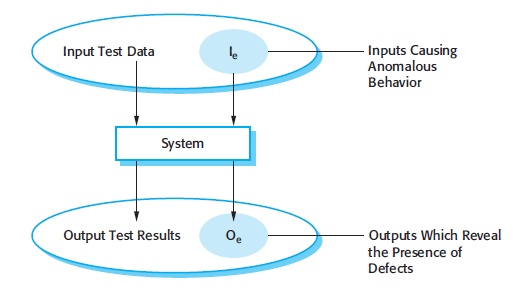
\includegraphics{modelo-teste.png}
	\label{fig:tipos-custo-arvore}
  \source{\cite{Sommerville2010}}
\end{figure}

\subsection{Caso de teste}
Um caso de teste  é um conjunto de possíveis entradas, condições de execução e resultados esperados de acordo com seus objetivos, estes quando compilados compõe uma instância única de execução em termos de entrada, execução e resultados esperados, estas saídas quando analisadas em relação aos dados esperados após execução determinam se o estado encontrado pela aplicação  é esperado \cite{Singh2014}. Os casos de teste são projetados para cenários particulares de teste aos quais é desejado comparar estados e resultados coletados a partir do resultado de sua execução com requisitos funcionais anteriormente definidos \cite{Jacob2016}.

\subsection{Mocks}
Ao construir testes automatizados é comum testar componentes de softwares que dependam de outros softwares , e desenvolvedores  normalmente necessitam testar o software com todas suas dependências ou simulações \cite{Spadini2017}. Ao testar todas as dependências juntamente, desenvolvedores passam a ter um comportamento similar ao ambiente de produção \cite{Spadini2017}.

Apesar dos benefícios, algumas dependências como bancos de dados e chamadas à serviços online podem ser custosos para serem testados, nestes casos desenvolvedores podem usar mocks \cite{Spadini2017}. Mocks são usados para substituir dependências reais em softwares ao simular suas características mais importantes, usualmente métodos em mocks  retornam valores desejados de acordo com os valores de entrada \cite{Spadini2017}. 

\subsection{Testes manuais}
O teste manual  é aquele executado através de um profissional de qualidade, o qual geralmente possui um caso de teste onde são descritos os passos de execução e por fim, o responsável toma decisões de acordo com a finalização da execução \cite{Kaprocki2015}.

Espera-se que os testes construídos para aplicações sejam, em geral, compostos pelos seguintes itens:

\begin{itemize}
	\item Estado inicial do teste;
	\item Eventuais entradas para uso;
	\item Sequência de passos para execução; 
	\item Uma ou mais saídas esperadas.
\end{itemize}

\subsection{Testes automatizados}

Os testes automatizados possuem uma estrutura comum aos testes manuais, porém o maior diferencial deste tipo de teste é delegar para a máquina a execução e possivelmente a validação dos resultados obtidos. Apesar de testes automatizados possuírem diversos papéis, como testes funcionais, testes de stress,é notório que estes possuam a capacidade de executar uma grande quantidade de casos de teste em um curto período de tempo, com maior precisão \cite{Kaprocki2015}.

\section{Teste caixa preta}

O teste caixa preta é uma categoria de testes funcionais a qual em sua execução não existe o conhecimento da estrutura interna do SUT \cite{Xu2016},  o conceito nasceu da ideia da estrutura interna do SUT estar coberta por uma caixa preta de maneira que o profissional de testes não tenha conhecimento de sua estrutura interna, somente de seu funcionamento, desta maneira o profissional de qualidade concentra no que o software deve fazer e elimina o raciocínio baseado na maneira como é feito \cite{Jacob2016}.

Geralmente ao efetuar um teste de caixa preta, o profissional de qualidade ou ferramentas de execução automatizada de scripts de teste poderão interagir com a interface de usuário de maneira que possam fornecer dados de entrada sem quaisquer noções da lógica de negócio por trás da interface utilizada \cite{Xu2016}. Idealmente este tipo de teste é guiado por especificações formais dos requisitos elicitados ou modelos de dados de teste, porém na prática estas especificações nem sempre estão disponíveis \cite{Walkinshaw2017}.

\section{Particionamento de equivalência}
O particionamento de equivalência é um critério de teste o qual divide o domínio possível de entradas do SUT em classes de dados as quais os casos de teste são derivados  \cite{Jacob2016}. Neste critério  todo o conjunto de entradas é particionado em subconjuntos ou classes, onde cada classe representa um conjunto de entradas similares para determinadas funcionalidades e especificações \cite{Jacob2016}.

O conceito por trás deste critério  é dividir as entradas de maneiras que os conjuntos façam parte de classes consideradas iguais, estes conjuntos são conhecidos como partições de equivalência ou classes de equivalência, desta maneira a quantidade de casos de teste  é menor dado que é necessário testar uma única condição para cada partição ou classe de equivalência \cite{Jacob2016}.

\section{Análise do valor limite}
A análise de valor limite é um critério similar ao critério de classe de equivalência no que diz respeito à estratégia de particionamento afim de diminuir a quantida de casos de teste necessários para cobrir um requisito, o seu ponto principal é dividir o domínio de uma ou mais entradas de maneira que diferentes faixas de valor possam ser representadas por uma quantidade menor de entradas, estas entradas compostas pelos valores limites das partições.

Segundo \cite{Jacob2016}, muitos dos desenvolvedores cometem erros ao implementar requisitos que dependem da utilização de valores limite para execução de asserções condicionais, desta maneira uma quantidade maior de defeitos ocorre nos valores limite de um domínio de entrada se comparado a defeitos que ocorrem por valores intermediáios da mesma faixa.

O profissional de qualidade deve estar alinhado com os seguintes princípios para mapear uma análise de valor limite:

\begin{itemize}
	\item Se a condição de uma entrada  é comprendida entre valores m e n, os casos de teste devem ser projetados para os valores m, n assim como entradas que representem os valores abaixo e assim de m e n, desta maneira o caso de teste deverá ser projetado para o conjunto de entradas {m,n,m};
\end{itemize}



\section{Qualidade de software e aspectos econômicos}

A Garantia de Qualidade ou \textit{Quality Assurance} é considerada uma das partes mais caras do desenvolvimento de software \cite{wagner2005}, o conceito de garantia de qualidade tornou-se mais evidente após a primeira conferência de engenharia de software com o propósito de estabelecer melhores princípios e estratégias econômicas para atingir um estado viável de software, esta conferência de em 1968 foi responsável	 inclusive a disciplina de teste e controle de qualidade em diversas  fases de desenvolvimento de software desde então \cite{repasi2009}.

De fato, os custos de garantia de qualidade são elevados \cite{wagner2005} \cite{Korel1990} já que consistem em todo e qualquer valor investido em atividades cujo propósito almeja qualidade de software \cite{pressman2009engenharia}, porém é notável que fatores econômicos em melhoria de qualidade não são bem aceitos por todos os interessados no desenvolvimento de software e que inclusive exista uma certa confusão sobre o valor de negócio da qualidade de desenvolvimento de software \cite{slaughter1998} já que teste de software é uma atividade trabalhosa e cara \cite{Korel1990} mas estes investimentos estes são importantes e devem ser planejados visto que cada valor gasto em horas de trabalho e não investido em retrabalho pode ser usado para melhorias rápidas em produtos e processo existentes \cite{slaughter1998}.

Os custos direcionados à qualidade de software são categorizados em \textit{conformance} e \textit{nonconformance} \cite{ slaughter1998}\cite{pressman2009engenharia} como demonstrado na figura a seguir: 

\begin{figure}[H]% H manda colocar exatamente nessa posição no texto (relativa aos parágrafos anterior e posterior)
	\centering
 	  \caption{Hierarquia da classificação dos tipos de custo presentes em desenvolvimento de software}
		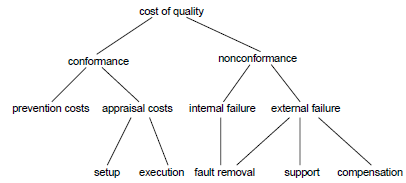
\includegraphics{tipos-custo-arvore.png}
	\label{fig:tipos-custo-arvore}
  \source{\cite{wagner2005}}
\end{figure}

Os custos de \textit{conformance} caracterizam os valores com o intuito de atingir maior qualidade de produto, este por sua vez é divido em custo de prevenção e custo de avaliação. \cite{ wagner2005}

Custos de prevenção são aqueles associados com o intuito de prevenir defeitos antes que possam ocorrer, geralmente são compreendidos por treinamentos, equipamentos, , revisões técnicas formais, atividades de planejamento de qualidade e reviews de produto \cite{wagner2005} \cite{pressman2009engenharia}.

Custos de avaliação compreendem custos relacionados a medidas e extração de métricas, avaliação e auditoria de produtos.\cite{wagner2005}, incluem atividades para ganhar conhecimento da condição do software em análise para cada início de ciclo, incluem: avaliações de processo e entre processos e manutenção \cite{pressman2009engenharia}.

Custos de não conformidade são os custos relacionados aos cenários em que não seguem o planejado e defeitos produzindo um erro e por fim levando à falha \cite{wagner2005}, nesta categoria estão as subcategorias de custos de falha externa e custos de falha interna \cite{pressman2009engenharia}. 

Os Custos de falha externa caracterizam os custos associados aos defeitos após liberação do produto de software para uso, são exemplos: Resolução de chamados, retorno e substituição de produtos e garantias \cite{pressman2009engenharia} enquanto os custos de falha interna são os custos aplicados para remoção de falhas antes de liberação para uso.

 O custo relativo para encontrar e reparar um defeito aumenta consideravelmente na linha do tempo entre as fases iniciais e finais do ciclo de desenvolvimento, sendo assim, custos do tipo \textit{nonconformance} se tornam mais caros ao longo do tempo de projeto, como demonstrado a seguir \cite{wagner2005}:

\begin{figure}[H]% H manda colocar exatamente nessa posição no texto (relativa aos parágrafos anterior e posterior)
	\centering
 	  \caption{Crescimento dos custos do tipo \textit{nonconformance} ao longo do tempo de projeto}
		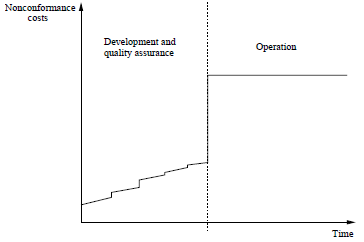
\includegraphics{nonconformance-costs-timeline.png}
	\label{fig:framework-teste}
  \source{\cite{wagner2005}}
\end{figure}

Apesar do custo relativo para encontrar e reparar um defeito aumenta consideravelmente na linha do tempo, o processo de desenvolvimento de um software flui entre os diversos ciclos, e por consequência, diferentes tipos de investimentos são feitos com o intuito de garantiar mainores níveis de qualidade \cite{pressman2009engenharia}. 





\chapter{Geração automática de dados de teste}
\label{chap:geracao-automatica-dados-teste}
A manutenção de softwares é usualmente vista não somente como uma tarefa difícil mas cara visto que as atividades ligadas à esta somam por volta de 60\% do investimento total de um software \cite{shamshiri2018}, concomitantemente os profissional de desenvolvimento de software necessitam testar o SUT utilizando-se de casos de teste que revelem falhas, aumentando a cobertura de caminhos e minimizando de custo e tempo simultaneamente. \cite{dave2015}.

O alto custo presente em testes de mutação e geração de mutantes pode ser reduzido pela geração automática de dados de teste \cite{dave2015}, a geração automática de testes poupa o tempo investido por desenvolvedores na escrita de testes unitários \cite{shamshiri2018}.

A geração automática de dados de teste consiste em uma tarefa importante no processo de testes de software, ela possui o objetivo de melhorar a qualidade de um determinado software under test (SUT) com o intuito de aumentar a qualidade do software e diminuir o custo investido.\cite{shamriski20151115}. A geração automática de dados de teste possui também um papel importante no processo de desenvolcimento de software visto que esta pode afetar diretamente a qualidade final de um produto de software \cite{dave2015}.

Os testes gerados podem ser incluídos nos repositórios de código do SUT como qualquer outro artefato de software \cite{shamshiri2018}, porém conjuntos de testes volumosos podem levar mais tempo para serem executadas e precisam ser avaliados antes de serem incluídos em uma suíte de testes \cite{shamriski20151115}. Ferramentas como a EvoSuite têm se mostrado eficazes em atingir alta cobertura de código em tiferentes tipos de softwares orientados a objetos. \cite{Campos2017}

A maneira mais fácil de avaliar conjuntos de testes automaticamente gerados é avaliar sua capacidade de expor falhas. \cite{shamshiri2018}, sendo assim, as avaliações de conjuntos de testes automaticamente gerados ocorre por meio de métricas como cobertura de linhas de código ou estimativas da habilidade de detecção de falhas, sendo um exemplo deste o score de mutação. \cite{shamshiri2018}





\section{Algoritmos baseados em busca}
Algoritmos baseados em busca têm se mostrado efetivos na geração de dados de teste quando otimizados para cobertura de código de diferentes tipos de software \cite{Campos2017} também mostraram-se eficazes quando aplicada para geração de suítes de testes unitários otimizados para cobertura de código em classes de softwares orientados a objetos\cite{Campos2017}

Novas técnicas de busca foram desenvolvidas nos últimos anos \cite{rojas2017b}, algoritmos de busca estão entre as técnicas mais bem sucedidas para automaticamente gerar dados de teste e testes unitários. \cite{rojas2017b}

Técnicas como buscas randômicas, buscas locais, simulated annealing e algoritmos genéticos são algumas das técnicas mais utilizadas. \cite{rojas2017b}

Uma abordagem popular é o uso de algoritmos evolutivos no qual os indivíduos utilizados ma população são testes os quais  após gerados compõe suítes de testes completas, a construção destas suítes ocorre com objetivo de encontrar suítes de teste os quais atingem a cobertura de código máxima a partir de técnicas baseadas em evolução natural \cite{Campos2017}

\section{Algoritmo baseado em busca aleatória}

O algoritmo de busca randômica, ou random search,  é um algoritmo o qual o mecanismo deve ser estabelecido para escolher os candidados em um espaço X, o processo randômico pode ser definido como a função de densidade de probabilidade P(x) a qual expressa a probabilidade de qualquer candidato presente em um espaço X de possíveis soluções \cite{Karnopp63}. Apesar de estudos na área, existe um número de técnicas padrão, técnicas como estas geralmente baseiam-se em um gerador randômico entre 0 e 1, o qual a saída pode ser utilizada para produzir uma aproximação da distribuição desejada. \cite{Karnopp63}

O algoritmo de busca randômica é um algoritmo o qual não utiliza operações de crossover, mutações ou selecões, ao contrário dos algoritmos genéticos seu funcionamento baseia-se puramente em estratégias de substituição \cite{Campos2017}. O algoritmo de busca randômica consiste em repetidamente gerar amostras de candidatos presentes em um espaço de busca de soluções possíveis para o problema a qual o candidato já presente na solução parcial é substituído se a aptidão do indivíduo gerado supera a aptidão do indivíduo já presente na resolução do problema em análise. \cite{Campos2017}

O Algoritmo de Random testing, é uma variação dos algoritmo baseado em busca aleatória o qual utiliza random search como base para construir suítes de testes de maneira incremental \cite{Campos2017} , esta diferencia-se das outras por gerar sequencias aleatórias de casos de teste juntamente aos dados de entrada também  aleatoriamente gerados \cite{shamriski20151115}, se um novo caso de teste gerado cobre um novo ramo do SUT o qual não foi coberto nas iterações anteriores, o novo caso de teste é adicionado ao conjunto  \cite{shamriski20151115}, os casos de testes são tradados como amostras individuais, se uma amostra gerada aumenta a cobertura de código, a amostra recém gerada é então inserida na suíte de testes, caso contrário é descartada. \cite{Campos2017}

Segundo \cite{Karnopp63} técnicas de busca randômicas possuem alguns vantagens de utilização como:

\begin{itemize}
	\item Facilidade de desenvolvimento: Por sua facilidade de programação do algoritmo, bons resultados podem ser obtidos com pouco esforço de desenvolvimento e algoritmos generalistas para resoluções de problemas de busca.
	\item Baixo custo: Os valores randômicoss utilizadas em buscas randômicas podem ser gerados com pouco custo computacional, muitos dos métodos necessitam meios de armazenamento e operações de comparação mutalmente simples.
	\item Eficiência: Em muitos casos, um algoritmo altamente de busca altamente randômico será muito mais eficiente se comparado a um algoritmo altamente determinístico, isto ocorre pois o tempo gasto em decidir a próxima estratégia de um algoritmo determinístico é investido em explorar e avaliar uma quantidade maior do universo de possíveis soluções.
	\item Flexibilidade: Algoritmos de busca randômicos possuem a flexibilidade de variar entre algoritmos puramente randômicos e altamente determinísticos de acordo com o problema em análise e o estágio de busca.
	\item Informação provida e utilizada: Algoritmos de busca randômicos podem coletar informações sobre a função de busca em execução e utilizar esta informação para guiar a busca, apesar destar informações serem do tipo local, podem ser utilizadas para otimização.
\end{itemize}


Em contraponto à facilidade de construção proporcionada pelo algoritmo de random search, possui a desvantagem do tamanho dos casos de testes gerados e consequentemente, o tempo de execução proporcionado pela execução e validação de cobertura destes. \cite{shamriski20151115}


Em contraponto à facilidade de construção proporcionada pelo algoritmo, este possui uma a desvantagem do tamanho dos casos de testes gerados e consequentemente, o tempo de execução proporcionado \cite{shamriski20151115}. A técnica de random search também é dificultada por valores de entradas os quais por determinados tipos de entrada como constantes, valores específicos de strings os quais não são difíceis de serem gerados sem algoritmos de seeding. \cite{shamriski20151115}


\section{Algoritmos de busca baseados em evolução}
Algoritmos evolutivos são inspirados na evolução natural, estes algoritmos têm se mostrado eficazes quando utilizados em diferentes tipos de problemas de otimização \cite{Campos2017}.

A população é gradualmente otimizada usando operações geneticamente inspiradas como a operação de crossover, esta operação combina material genético de no mínimo dois indivíduos para assim gerar uma nova prole , e mutação, uma operação na qual troca altera material genético em um indivíduo a uma baixa probabilidade, para assim garantir diversificação genética \cite{Campos2017}. No contexto de geração de suítes de teste, os indivídios da população são caracterízados por conjuntos de casos de teste, também chamados de suítes de teste. \cite{Campos2017}


A seleção de indivíduos é guiada por uma função de aptidão, a qual pontua melhor  os indivídios mais adaptados para um problema de otimização \cite{Campos2017}. A função de aptidão baseia-se em objetivos decobertura que vão da cobertura de código a cobertura de ramificações de código \cite{Campos2017}, sendo assim indivíduos com valores altos de aptidão são mais adaptados ao problema em questão e mais prováveis de sobreviver a novas iterações e produzirem novos candidatos. \cite{Campos2017}

O aumento do número de objetivos de cobertura pode afetar a performance do algoritmo evolutivo \cite{Campos2017}

\subsection{Algoritmos genéticos}

Os algoritmo genéticos estão entre os algoritmos evolutivos mais usados em diversos problemas de otimização pois podem ser fácilmente implementados e apresentam bons resultados  \cite{Campos2017}.  No contexto de geração de suítes de testes e algoritmos genéticos, os indivídios da população são caracterízados por conjuntos de casos de teste, também chamados de suítes de teste \cite{Campos2017}. Os algoritmos genéticos geralmente possuem os seguintes passos lógicos: \\



\begin{algorithm}[htbp]
\caption{Algoritmo genético padrão com as seguintes entradas: Condição de parada $C$, função de aptidão $A$, função de seleção $Fs$, tamanho de população $Tp$, função de crossover $Fc$, probabilidade de crossover $Pc$, função de mutação $Fm$ e probabilidade de mutação $Pm$.}
\label{alg:algoritmo-genetico}


\begin{algorithmic}[1]

\State$ P \leftarrow  PopulacaoRandomicamenteGerada(ps)$ \label{ga:line:rand}
\State ValidarAptidão(ps)
\State \textbf{Enquanto} $\neg C$ \textbf{faça}
\State \quad $ Np \leftarrow  []$
\State \quad \textbf{Enquanto} $ |Np| < Tp $ \textbf{faça}
\State \quad \quad  $ p1,p2 \leftarrow Selecionar(Fs, P) $ \label{ga:line:selecionar}
\State \quad \quad  $ o1,o2 \leftarrow Crossover(Fc, Pc, p1,p2) $ \label{ga:line:crossover}
\State \quad \quad  $ Mutacao(Fm, Pm, o1) $ \label{ga:line:Mutacao}
\State \quad \quad  $ Mutacao(Fm, Pm, o2) $ \label{ga:line:Mutacao2}
\State \quad \quad  $ Np \leftarrow  Np \cup \{o1,o2\}$
\State \quad \textbf{Fim enquanto}

\State  $ P\leftarrow  Np$
\State ValidarAptidão($A$,$P$) \label{ga:line:aptidao1}
\State \textbf{Fim enquanto}
\State \textbf{retornar} $P$

\end{algorithmic}
\source{\cite{Campos2017}}
\label{alg:algoritmo-GA}
\end{algorithm}

No algoritmo \ref{alg:algoritmo-GA} é possível verificar os passos de execução na versão padrão do algorítmo, o algoritmo começa gerando uma população randômica de indivíduos os quais são potenciais soluções para o problema em análise (linha \ref{ga:line:rand}). Sem seguida, enquanto a condição de parada $C$ não for atingida, os seguintes passos serão executados para cada indivíduo : seleção (linha \ref{ga:line:selecionar}), crossover (linha \ref{ga:line:crossover}) e mutação (linhas \ref{ga:line:Mutacao} e \ref{ga:line:Mutacao2}). Por fim, a cada uma dessas iterações, a funcão de aptidão é aplicada (linha \ref{ga:line:aptidao1}) com o intuito de pontuar indivíduos com a melhor aptidão para resultado na solução em questão para que estes não sejam descartados na função de selecão da próxima iteração linha(\ref{ga:line:selecionar}). 

Diversas variações do algoritmo genético padrão foram propostos com o intuito de melhorar sua efetividade \cite{Campos2017}. Uma das variações de algoritmo genético é sua versão monotônica do algoritmo genético padrão (Standard GA), a versão monotônica somente inclui, após operações de mutação e validação em cada iteração, somente o melhor conjunto da prole ou o melhor indivíduo da prole anterior \cite{Campos2017}.  Dentre as variações de algoritmos genéticos padrão, existe a variação Steady State GA, esta variação utiliza a mesma estratégia de substituição presente na variação monotônica, a prole descendente substitui os ascendentes da população atual imediatamente a ocorrência da fase de mutação.  \cite{Campos2017}


\subsubsection{O algoritmo evolutivo 1 + ($\lambda$,$\lambda$)}
A versão do algoritmo evolutivo 1 + ($\lambda$,$\lambda$) , introduzida por Doerr, possui como primeiro passo a geração de uma população randômica de tamanho 1, em seguida, a operação de mutação é aplicada afim de criar $\lambda$ versões diferentes com mutação do indivíduo em análise \cite{Campos2017}. A alta probabilidade de mutação ocorre para incentivar que a exploração seja mais rápida no expaço de busca disponível. \cite{Campos2017}

No próximo passo, o operador de mutação é aplicado novamente com uma probabilidade maior de mutação, dada por K, onde K é usualmente maior que um, isto permite que, na maioria dos casos, mais de um gene seja mutado por cromossomo. Por fim, a operação de crossover acontece uniformemente aos ascendentes e aos melhores descendentes para criar uma prole de  tamanho $\lambda$  \cite{Campos2017}. A operação de crossover unificada entre o melhor indivíduo com os lambda mutantes e seu ascendente foi proposta para amenizar os defeitos causados pela mutação agressiva, após essa operação, toda a prole e avalidada e somente o melhor indivíduo é selecionado \cite{Campos2017}

Se o melhor descendente é melhor avaliado do que o seu ascendente, a população criada de tamanho um é então substituída pela melhor prole. \cite{Campos2017}

\subsubsection{O algoritmo evolutivo  $\mu$ + $\lambda$}

O algoritmo evolutivo $\mu$ + $\lambda$  é um algoritmo baseado em mutações onde o número de ascendentes e descendentes são restringidos respectivamente  a $\mu$ e $\lambda$ \cite{Campos2017}. Cada gene sofre mutação independente com probabilidade 1/n, após a operação de mutação, a prole gerada é comparada com cada asendente com o intuito de manter os melhores ascendentes presentes até então \cite{Campos2017}.

Entre as diferentes versões do algoritmo, existem duas melhores configurações como (1+$\lambda$) e (1+1) os quais a população tem tamanho 1 e o número da prole é limitado a 1 no caso de parâmetros (1+1) \cite{Campos2017}.

\subsubsection{O algoritmo evolutivo MOSA}
O algoritmo MOSA, Many-Objective Sorting Algorithm, contrapõe os outros algoritmos por tratar cada objetivo de cobertura como um objetivo de otimização independente \cite{Campos2017}. Este algoritmo é uma variação do algoritmo NSGA-II o qual melhor avalia os melhores testes gerados por cada objetivo de cobertura antes não coberto, independente da relação entre os testes e a população. \cite{Campos2017}

Para que seja possível trabalhar com o grande número de objetivos de cobertura, o qual ocorre por conta da combinação dos diversos objetivos de cobertura, a extensão  do algoritmo DynaMOSA dinamicamente seleciona  os critérios  \cite{Campos2017}. Tanto o algoritmo MOSA quanto o algoritmo DynaMOSA demonstraram atingir alta cobertura de alguns critérios selecionados quando comparados aos algoritmos genéticos tradicionais. \cite{Campos2017}

\section{Algoritmo de busca randômica ou algoritmos evolutivos ?}
Apesar de muitos dos aspectos destes algoritmos avaliados em detalhes, a influência de diferentes algoritmos em diferentes casos recebeu pouca atençãona literatura \cite{Campos2017}. Vários algoritmos foram propostos porém nenhum dos algoritmos pode ser considerado melhor em todos os domínios de problemas , alguns algoritmos performam melhor do que outros de acordo com as características presentes no domínio do problema. \cite{Campos2017}


É teoricamente impossível desenvolver um algoritmo de geração de dados de teste o qual performa bem em todos os tipos de problemas disponíveis \cite{Campos2017}. Uma abordagem comum em problemas de geração de dados de testes na engenharia de software é utilizar um algoritmo genético primariamente e somente depois refiná-lo ou compará-lo com outros algoritmos para assim verificar qual dos algoritmos e soluções disponíveis  é apropriado para o problema em questão. \cite{Campos2017}

O estudo promovido por \cite{Campos2017} demonstra que algoritmos genéticos claramente performaram melhor do que algoritmos randômicos, em média os evolutional algorithms possuem maior cobertura quando comparados a random search e random testing. \cite{Campos2017}

\cite{Campos2017} afirma a necessidade compreender as diferentes características de software as quais influenciam diferentes coberturas de teste nas diferentes técnicas para que assim seja possível desenvolver uma hyper-heurística a qual seleciona a adapta o algoritmo para cada problema de geração em específico.

\section{EvoSuite}
Existem várias ferramentas de geração de dados de testes com base em buscas disponíveis em uma gama de linguagens de programação, principalmente Java e .NET. Ferramentas as quais variam de técnicas de random search como Randoop, Jcrasher, JTExpert, NightHawk, T3 ou Yeti-Test até ferramentas baseadas em técnicas evolutivas como EvoSuite, eToc ou Testful. \cite{shamriski20151115}

A EvoSuite \cite{Evosuite} é uma ferramente baseada em técnicas de busca que também utiliza algoritmos genéticos na geração automatica de suítes de testes para classes escritas em Java. \cite{Fraser2017}. Para uma determinada classe, referenciada na ferramenta como alvo, e seu classpath completo, o caminho o qual o ambiente de execução possa encontrar as classes compiladas como bytecode e respectivas dependências \cite{ClassPath}, a EvoSuite automaticamente produz um conjunto de testes unitários escritos para o framework de execução de testes Junit \cite{Junit} com o intuito de maximixar a cobertura de código. \cite{Fraser2017}.

A efetividade da EvoSuite tem sido avaliada tanto como uma ferramenta opensource quanto uma ferramenta de apoio a testes nas áreas industriais se tratando de cobertura de código, efetividade na busca de falhas e inclusive aumentando a produtividade de desenvolvimento \cite{Fraser2017}. 

A ferramenta conseguiu o primeiro lugar nas segunda e quarta edições do unit testing tool competition além de conseguir o segundo lugar na terceira edição \cite{Fraser2017}, a configuração da EvoSuite para a competição em maioria manteve seus valores padrão, já que estes foram ajustados extensivamente \cite{Fraser2017}. Com um budget de 480 segundos, a ferramenta atingiu em média 66.5\% de cobertura de caminhos, 0.9\% superior se comparado ao ano anterior com um score de mutação de 50.7\%, 9.7\% super do que o ano anterior. \cite{Fraser2017}

Além das últimas melhorias, diversas correções foram aplicadas desde a última edição do unit testing tool competition em 2017  \cite{Fraser2017}, no ano de 2017 a ferramenta passou a utilizar mocks em seus testes através da ferramenta Mockito \cite{Mockito} \cite{Fraser2017}. Após atingir determinada porcentagem do tempo de busca disponível, a ferramenta considera o uso de mocks ao invés de classes reais, somente caminhos que não puderam ser cobertos por meio de mocks resultaram com o uso de mocks.  \cite{Fraser2017}


\chapter{Métricas de Softwares orientados a objetos}
\label{chap:metricas}

Projeto e desenvolvimento de softwares orientados a objeto são conceitos populares no cenário atual de desenvolvimento de software \cite{srivastava2013}, neste contexto é notável que classes e métodos são estruturas básicas neste gênero de software \cite{kan95}. O desenvolvimento de software orientado a objetos difere de outros paradigmas pois requer uma abordagem voltada para regras de negócio completamente diferente das tradicionais, dado na maneira como a decomposição funcional e fluxo de dados ocorrem  \cite{srivastava2013}.

A análise e projeto de softwares orientados a objeto focam nos objetos como estruturas primárias de computação \cite{kan95} \cite{srivastava2013}, nesta cada classe é composta por dados e operações realizadas, os quais  são representações de uma única entidade real de negócio \cite{srivastava2013}.

As operações realizadas são caracterizadas pelos métodos das classes, a quantidade de funcionalidade, representada por método, agregada ao um software orientado a objeto pode ser estimada com base na quantidade de classe, métodos e variantes destes, utilizados \cite{kan95}. Desta maneira, é comum relacionar métricas de softwares orientados a objeto a valores baseados em atributos de classes e métodos, sejam linhas de código, complexidade, entre outros \cite{kan95}.

As métricas de software tornaram-se elementos primordiais em diversos domínios de Engenharia de software, e principalmente no âmbito de garantia de qualidade, já que toda a informação reúnida por métricas pode ser submetida à diversos tipos de análise e comparação com dados históricos com o objetivo de avaliar e garantir qualidade de software \cite{srivastava2013}. Métricas de software podem ser utilizadas para predizer atributos de qualidade em tempo de execução, inclusive para aplicações cujo requisito é ser uma aplicação de tempo real \cite{srivastava2013}. O real valor de métricas de software vem da sua representação dos atributos de software externos, muitos destes com alto valor de negócio, como confiabilidade, mantenibilidade, reusabilidade, testabilidade e eficiência \cite{srivastava2013}, os quais são requisitos de qualidade descritos pela ISO9126 \cite{Zeiss2007}.



%Um grande número de métricas foi proposto ao longo do tempo pela literatura \cite{srivastava2013}.



\section{Medidas diretas e indiretas}
Uma medida direta de software é uma métrica a qual o cálculo de seu valor não depende nenhum outro atributo além do principal utilizado em seu cálculo \cite{srivastava2013}. Exemplos claros de medidas em produtos são: LOC (\textit{Lines of code}), velocidade de execução, tamanho de memória, quantidade de defeitos reportados \cite{srivastava2013}.

Uma medida indireta de software é uma métrica a qual envolve a medida de um ou mais atributos de software\cite{srivastava2013}. As medidas diretas são, em geral, mais fáceis de serem coletadas.


\section{O conjunto de métricas CK}

Em 1994 Chidamber e Kemerer proporam seis métricas de projeto e complexidade de softwares orientados a objeto, as quais, futuramente, tornaram-se o conjunto de métricas CK \cite{kan95}. 

Chidamber e Kemerer aplicaram as seis métricas do conjunto (as quais serão definidas em seções posteriores) em estudos empíricos de duas empresas, uma usando C++ e outra Smalltalk \cite{kan95}, o sumário desta é demonstrado na tabela.

\subsection{\textit{Weighted methods per class (WMC)}}
A WMC é uma métrica contabilizada pela soma das complexidades dos métodos, onde a complexidade é dada pelo \textit{cyclomatic complexity number}  de McCabe (CCN)\cite{kan95} \cite{watson96}. Medir o \textit{cyclomatic complexity number} não é trivial de implementação dado que nem todos os métodos são acessíveis de acordo com a hierarquia dos objetos, isso é resultado por conta da herança aplicada no projeto do componente \cite{kan95}.

\subsection{\textit{Depth of inheritance tree (DIT)}}
A DIT é uma medida que compreende o valor do comprimento máximo de um caminho em uma árvore de herança, este comprimento é dado pela distância entre o nó em análise até o nó raíz \cite{kan95}. A definição da DIT baseia-se na premissa de que desenvolvedores lidam com linguagens de programação orientadas a objeto as quais permitam que uma classe possua no máximo uma classe pai \cite{bruntink04}, linguagens alheias a este conceito são conhecidas por possuir herança múltipla, presente em linguagens como C++ e Python. Muitas linguagens orientadas a objeto não suportam herança múltipla por conta do problema do diamante, supondo a estrutura a seguir:

\begin{figure}[H]% H manda colocar exatamente nessa posição no texto (relativa aos parágrafos anterior e posterior)
	\centering
 	  \caption{Exemplo de problema do diamante}
		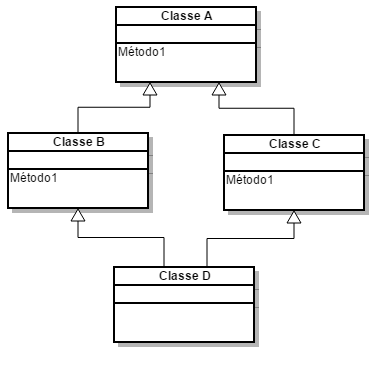
\includegraphics{diagrama_diamante.png}
	\label{fig:tipos-custo-arvore}
  \source{Gustavo Ramos, 2017}
\end{figure}

Neste caso, um objeto instanciado do tipo D possui acesso para executar o \textbf{Método 1}, porém o compilador pode não saber a qual referência de \textbf{Método 1} executar já que o objeto do tipo D herda tanto de B e de C quanto de A, todos os quais possuem o \textbf{Método 1}. Este caso é conhecido por problema do diamante, por conta deste, linguagens como Java não permitem a herança múltipla.Dada a premissa de que a linguagem do software em análise não suporta herança múltipla, ao calcular o DIT, o número de ancestrais do nó $c$ em análise, corresponde à profundidade de $c$ na árvore de herança \cite{bruntink04}. A fórmula que descreve o cálculo da DIT para um determinado nó $c$ é dado a seguir:

\begin{equation}
  DIT(c) = |Ancestrais(c)|
	\label{eq:calc-dit}
\end{equation}

\subsection{\textit{Number of children of a class (NOC)}}

O NOC é uma métrica de simples cálculo, caracterizada pelo número de sucessores imediatos(subclasses) na árvore de hierarquia, calculada com base em  uma classe $c$ em análise \cite{kan95}. Seu cálculo é dado pela fórmula a seguir:

\begin{equation}
  NOC(c) = |Filhos(c)|
	\label{eq:calc-noc}
\end{equation}


\subsection{\textit{Coupling between object classes (CBO)}}
Uma classe $A$ é acoplada a uma classe $B$ se a classe $A$ invoca uma método ou utiliza uma variável de uma instância de $B$ \cite{kan95}, sendo assim, o CBO é dado pelo número de classes a qual uma classe $c$ em análise está acoplada, ou seja, seu cálculo é dado por:

\begin{equation}
  CBO(c) = |Quantidade de classes que relaciona(c)|
	\label{eq:calc-cbo}
\end{equation}

\subsection{\textit{Response for a class (RFC)}}
O RFC é caracterizado pelo número de métodos que podem ser executados na resposta de uma mensagem recebida por uma instância de uma classe \cite{kan95}, ou seja, o RFC é uma contagem do número de métodos de uma classe $c$ em análise e o número de métodos de outras classes que são invocados pelos métodos de $c$ \cite{bruntink04}.

Quanto maior o número de métodos que podem ser invocados indiretamente através de uma chamada de um método, maior a complexidade de uma classe, basicamente o RFC captura o tamanho de conjunto de respostas de uma classe \cite{kan95}. O RFC é calculado pelo número de métodos locais mais o número de métodos chamados por métodos locais \cite{kan95}.


\subsection{\textit{Lack Of Cohesion Of Methods (LCOM)}}
A independência pode ser medida por critérios qualitativos: coesão e acoplamento, a coesão é a medida relação funcional de um módulo \cite{pressman2009engenharia}, neste contexto, a coesão de uma classe é dada pela proximidade de métodos locais à instâncias de variáveis na classe, alta coesão indica uma boa subdivisão das classes \cite{kan95}.

A métrica LCOM representa a dissimilaridade dos métodos em uma classe pelo uso de instâncis de variáveis, a alta de coesão aumenta a complexidade e por consequência, oportunidade de ocorrência de erros durante o processo de desenvolvimento \cite{kan95}.

\section{Modelo proposto por Srivastava e Kumar}

Srivastava e Kumar proporam em 2013 um modelo de métricas para validação de qualidade de software com a justificativa de que nenhuma das métricas tratavam acoplamento ou similaridades como relações transacionais, sendo assim, métricas que mapeiam estas características são passíveis de incorporação no modelo. No estudo em questão, diversos dados foram coletados de projetos orientados a objeto nas linguagens Java e C++ e neste constatado que diversas métricas são baseadas em ideias similares e representam informações redundantes, sendo assim, foi validado que um subconjunto de métricas pode ser utilizado para predição de falhas.

O modelo proposto por \cite{srivastava2013} atingiu um nível de acurácia superior a 80\% na predição de falhas em classes.

\begin{figure}[H]% H manda colocar exatamente nessa posição no texto (relativa aos parágrafos anterior e posterior)
	\centering
 	  \caption{Modelo de qualidade proposto por Srivastava e Kumar}
		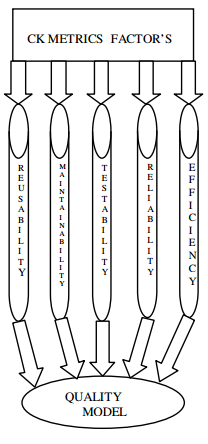
\includegraphics{modelo_srivastava_kumar.png}
	\label{fig:tipos-custo-arvore}
  \source{\cite{srivastava2013}}
\end{figure}

É observado na literatura que métricas de softwares orientados a objetos aliadas aos modelos de classificação e predição existentes possuíram efetividade em encontrar relação entre identificação e classificação de falhas e qualitdade de software  \cite{Suresh2016}. O fato ocorre pois métricas de software são a melhor ferramenta para avaliar a qualidade de softwares orientados a objetos.  \cite{Suresh2016}

É observado que muitos conjuntos de métricas disponíveis provém informações de qualidade de softwares orientados a objetos.  \cite{Suresh2016}


\section{Métricas extraídas com o SB4SE}
Além de características que possam ser descritas por métricas C.K, é possível também utlizar métricas as quais descrevam características de métodos, já que métodos compõe as ações  presentes dem classes.  No traballho desenvolvido por \cite{Eler2016}, diversas métricas de métodos foram extraídas utilizando execução simbólica, métricas como: Número de loops (NLp)número de loops aninhados (NNLp); quantidade de constantes (NCtt); número de variáveis (NVar); quantidade de variáveis do tipo inteiro (NInt);  quantidade de variáveis do ponto flutuante (NFit); quantidade de referências nulas (NNull); Quantidade de variáveis do tipo string (NStr); número de objetos (NObj); Número de arrays (NArr).

\chapter{Mineração de dados}

Mineração de dados é o processo de extrair conhecimento valioso de um grande agrupamento de dados, desconhecido e de valor para o problema em questão \cite{Seth2016, sharma2015}, processo este onde ocorre a análise de dados a partir de diferentes perspectivas, sumarizando com o intuito de obter informaçãos úteis para tomada de decisão  \cite{ sharma2015}. Ela é utilizada em diversos campos como robótica, decisões de marketing, decisões corporativas, inteligência de negócio e segurança \cite{ Seth2016}.

Na área de mineração de dados, distinguir diferentes classes a partir de um volume de dados e classificar a partir destes é uma técnica importante \cite{Seth2016}, sendo assim, a classificação é uma subárea de mineração de dados importante, dado que ela é capaz de analisar dados e organizá-los em classes a partir de suas características \cite{ Seth2016}.

\section{Classificação}
A classificação é uma técnica vastamente utilizada no domínio de mineração de dados, onde escalabilidade e eficiência são requisitos imediatos em classificação de grandes conjuntos de dados \cite{sharma2015}. A classificação é uma atividade não supervisionada \cite{ sharma2015},  a qual já existe o conhecimento desde o início quais são as classesdisponíveis a serem utilizadas pelo algoritmo, oalgoritmo então usa a informação de classes e características presentes em um dataset para treinamento e validação \cite{ sharma2015}.

Um problema de classificação é conhecido estruturalmente por receber uma entrada de dados, conhecido por conjunto de dados de aprendizagem (dataset), o qual é caracterizado por uma série de características (features) de análise e respectivas classes \cite{ Seth2016}. 

O principal objetivo de algoritmos de classificação é construir um modelo de classificação utilizando o conhecimento obtido a partir do conjunto de dados de aprendizagem e avalidar uma porcentagem desdes a partir do conhecimento adquirido. \cite{ Seth2016}

Diferentes algoritmos de classificação usam diferentes técnicas para encontrar relação entre os dados e as classes  \cite{ sharma2015}, estas relações estão sumarizadas em um modelo, o qual pode ser aplicado em novas instâncias para assim classifica-las.  \cite{ sharma2015}

Um modelo pode também ser utilizado para validação, onde novas instâncias são submetidas a um modelo e avaliadas em seguida para verificar se foram classificadas corretamente, este processo é chamado de validação do modelo  \cite{ sharma2015}.

Dentre os classificadores mais famosos, o mais conhecido é o classificador bayseano. \cite{ Seth2016}, o classificador bayseano é um classificador construído com base no teorema de bayess. \cite{ Seth2016}

Quando aplicado a grandes datasets, classificadores bayseanos provem alta acurácia em alta velocidade. \cite{ Seth2016}, a forma mais simples de classificador bayseano conhecido atualmente é o Classificador naive bayes. \cite{ Seth2016}

\section{Classificador naive bayes}

O teorema bayseano deriva da estatística bayseana, o qual possui premissas fortes e ingênuas \cite{Suresh2016}. O classificador bayseano é uma abordagem probabilística simples o qual assume que todos os atributos de um tupla pertencem a uma dada classe com uma probabilidade independente de ser classificado em relação a outros atributos  \cite{Suresh2016}.
 
O teorema bayseano é uma afirmação estatística que permite o cálculo de probabilidades condicionais, probabilidades condicionais são probabilidades que refletem a influência de um evento na probabilidade de outro evento  \cite{ sharma2015} .

Os termos geralmente utilizados em estatística bayseana são: probabilidade anterior e posterior: A probabilidade anterior é o evento com sua probabilidade original, antes de obter qualquer informação adicional em contraponto, a probabilidade posterior é a probabilidade anterior seguida de alguma informação adicional  \cite{ sharma2015}. O teorema de bayes pode ser descrito como  \cite{ sharma2015}:

\begin{equation}
P(A|B) = \frac{P(B|A).P(A)}{P(B)}
\end{equation}

Onde:\\
P(A) é a probabilidade anterior de A\\
P(B) é a probabilidade anterior de B\\
P(A|B) é a probabilidade posterior de A dado B\\
P(B|A) é a probabilidade posterior de B dado A\\

O classificador naive bayes funciona da seguinte maneira \cite{ Seth2016}:

\begin{enumerate}
  \item Inicialmente é necessário um conjunto de treinamento C com k caraterísticas e classes associadas, usando o valor de atributos presente em cada tupla do dataset, caracterizado por um vetor $\alpha$=($\alpha$1, $\alpha$2, $\alpha$3,…., $\alpha$k);
  \item A partir de um conjunto um conjunto de M classes beta compostos por $\gamma$1, $\gamma$2, $\gamma$3,…., $\gamma$m; O papel do classificador é predizer a partir de uma tupla $\alpha$ qual a classe  $\gamma$ com maior probabilidade a qual esta tupla pertence dado o que foi aprendido com o conjunto de treinamento, ou seja, o classificador prediz se uma tupla $\alpha$i pertence a uma classe $\gamma$i a partir da seguinte fórmula:
  
\begin{equation}
P(yi|alpha) > P(yj|alpha)\textrm{, para todo 1 $\leq$ j $\leq$ m, j $\neq$ i}
\end{equation}

\end{enumerate}

Consequentemente, P($\gamma$i|$\alpha$)  deve ser maximizado, a classe resultante com o maior valor de P($\gamma$i|$\alpha$)  é chamada de probabilidade posterior, como no teorema de bayes.Dado o fato de que para todas as classes P($\alpha$) é constante, maximizar P($\alpha$|yi) * P(yi) garante o propósito \cite{ sharma2015}.

Um conjunto de treinamento com muitos atributos para o cálculo de P($\alpha$) pode ser computacionalmente custoso de ser calculado, sendo assim, o classificador reduz este custo assumindo que as classes são condicionalmente independentes entre si \cite{ sharma2015}.


\section{Weka}
A ferramenta Weka (Waikato Environment for Knowledge Learning) é um software desenvolvido pela universidade de Waikato na nova zelândia \cite{Subbulakshmi2012}.  A WEKA suporta diferentes tipos de atividades como pré processamento, classificação, clusterização, regressão, visualização e seleção de atributos \cite{Subbulakshmi2012}. A premissa da aplicação é utilizar-se de um computador e o software para executar técnicas de aprendizado de máquina e mineração de dados e derivar informações úteis através de padrões \cite{Subbulakshmi2012}.

A feramenta possui em torno de duas décacas, com  implementações dos algoritmos de classificação com interfaces gráficas de fácil uso e visualização além de algoritmos de validação \cite{Bouckaert2008}. 

A Weka opera com dados unidimensionais, permitindo que pessoas de qualquer nível de conhecimento em mineração de dados  possam identificar informações escondidas em seus conjuntos de treinamentos com uma interface simples e direta \cite{Subbulakshmi2012}.  Após carregar e treinar um modelo com um conjunto de dados, o classificador pode ser validado para o conjunto e as classes fornecidas \cite{Subbulakshmi2012}. 

\chapter{Resultados e Discussões}
\label{chap:resultados}
Neste capítulo serão apresentados os resultados obtidos por meio das informações encontradas e dos testes aplicados durante o desenvolvimento da pesquisa. Para efeito de organização, este capítulo será dividido em seções que explicam desde os materiais e métodos utilizados até os resultados obtidos, dados gerados, assim como as conclusões extraídas e trabalhos futuros.

\section{Materiais}

Durante o processo de pesquisa, foi utilizado um conjunto de 110 projetos os quais são reconhecidos e utilizados por diversos pesquisadores da área. Os projetos em questão fazem parte do corpus SF110, o qual é caracterizado por um conjunto de 110 projetos open source retirados do site SourceForge\footnote{https://sourceforge.net/} compostos por: 100 projetos aleatoriamente escolhidos somados a  10 dos projetos com mais download em junho de 2014. \cite{shamriski20151115}.

O corpus SF110 foi utilizado como objeto de análise pelo processo de pesquisa por conta de sua diversidade de características, isso ocorre pois os projetos que compõe o corpus resolvem problemas presentes em domínios variados.  A partir do corpus, diversas ferramentas foram utilizadas para extrair informações e processá-las, o uso destas será detalhada na seção de métodos, para este processos as seguintes ferramentas foram utilizadas 



\begin{itemize}
  \item \textbf{EvoSuite\footnote{http://www.evosuite.org/}:} ferramenta utilizada para geração dos dados de teste nas duas técnicas apresentadas no capítulo 2 e cálculo da porcentagem de cobertura de código atingida;
  \item \textbf{CK\footnote{https://github.com/mauricioaniche/ck}:} ferramenta disponível em repositório opensource para extração de métricas CK em projetos Java;
  \item \textbf{Weka\footnote{https://www.cs.waikato.ac.nz/ml/weka/}:} ferramenta de mineração de dados utilizada para classificação pela técnica citada no capítulo 5;
  \item \textbf{LibreOffice Calc\footnote{https://www.libreoffice.org/discover/calc/}:} ferramenta utiizada para o cálculo das correlações entre os valores que serão apresentados.
  \item \textbf{Go \footnote{https://golang.org/}:} linguagem de programação utilizada para codificação de algumas rotinas de processamento dos dados.
  \item \textbf{Maven \footnote{https://maven.apache.org/}:} ferramenta de compilação, gestão de dependências e empacotamento dos projetos java presente no SF110.
\end{itemize}

Nas seções posteriores será descrita a metodologia aplicada durante o processo de pesquisa e os resultados encontrados, o processo foi segmentado nas tarefas de extração e análise das métricas, geração dos dados de teste, associação dos resultados, mineração dos dados, teste da hipótese e análise dos resultados.
 
  \section{Extrações de dados a análises primárias}
  A primeira etapa do processo consistiu na  extração dos dados para análises primárias das hipóteses apresentadas, este passo foi necessário pois a primeira análise estatística  para validação foi a análise da correlação das métricas CK dos projetos e os dados de execução fornecidos da EvoSuite: Cobertura de código e tempo de execução. A análise da correlação é uma etapa de validação importante visto que valores de correlação com pouca ou nenhuma significância podem dar indícios da eficácia de seu uso na mineração de dados, esta etapa caracteriza como uma etapa eliminatória das etapas posteriores do processo. 
  
 Os dados necessários para a análise da correlação são as devidas quantidades de cobertura, tempo disponibilizados pela EvoSuite e métricas CK extraídas das classes do SF110. Por conta da velocidade de extrair métricas estáticas como as métricas CK, a primeira coleta ocorreu com a geração dos dados de teste pela EvoSuite, inicialmente com o algoritmo de busca genético padrão e em seguida com o algoritmo de busca randômica.
 
 O SF110 possui em torno de <X> classes java, espera-se então que o conjunto de dados consolidado final para treinamento possua o mesmo número, porém alguns dos projetos apresentaram problemas ao serem compilados , outros apresentaram mensagens de erro ao iniciar a geração de dados de testes utilizando algoritmos genéticos por meio da EvoSuite e alguns projetos possuíram tempo de execução superior a 8 horas.



\begin{figure}[H]% H manda colocar exatamente nessa posição no texto (relativa aos parágrafos anterior e posterior)
	\centering
 	  \caption{Distribuição de estado dos projetos após geração de dados de teste}
		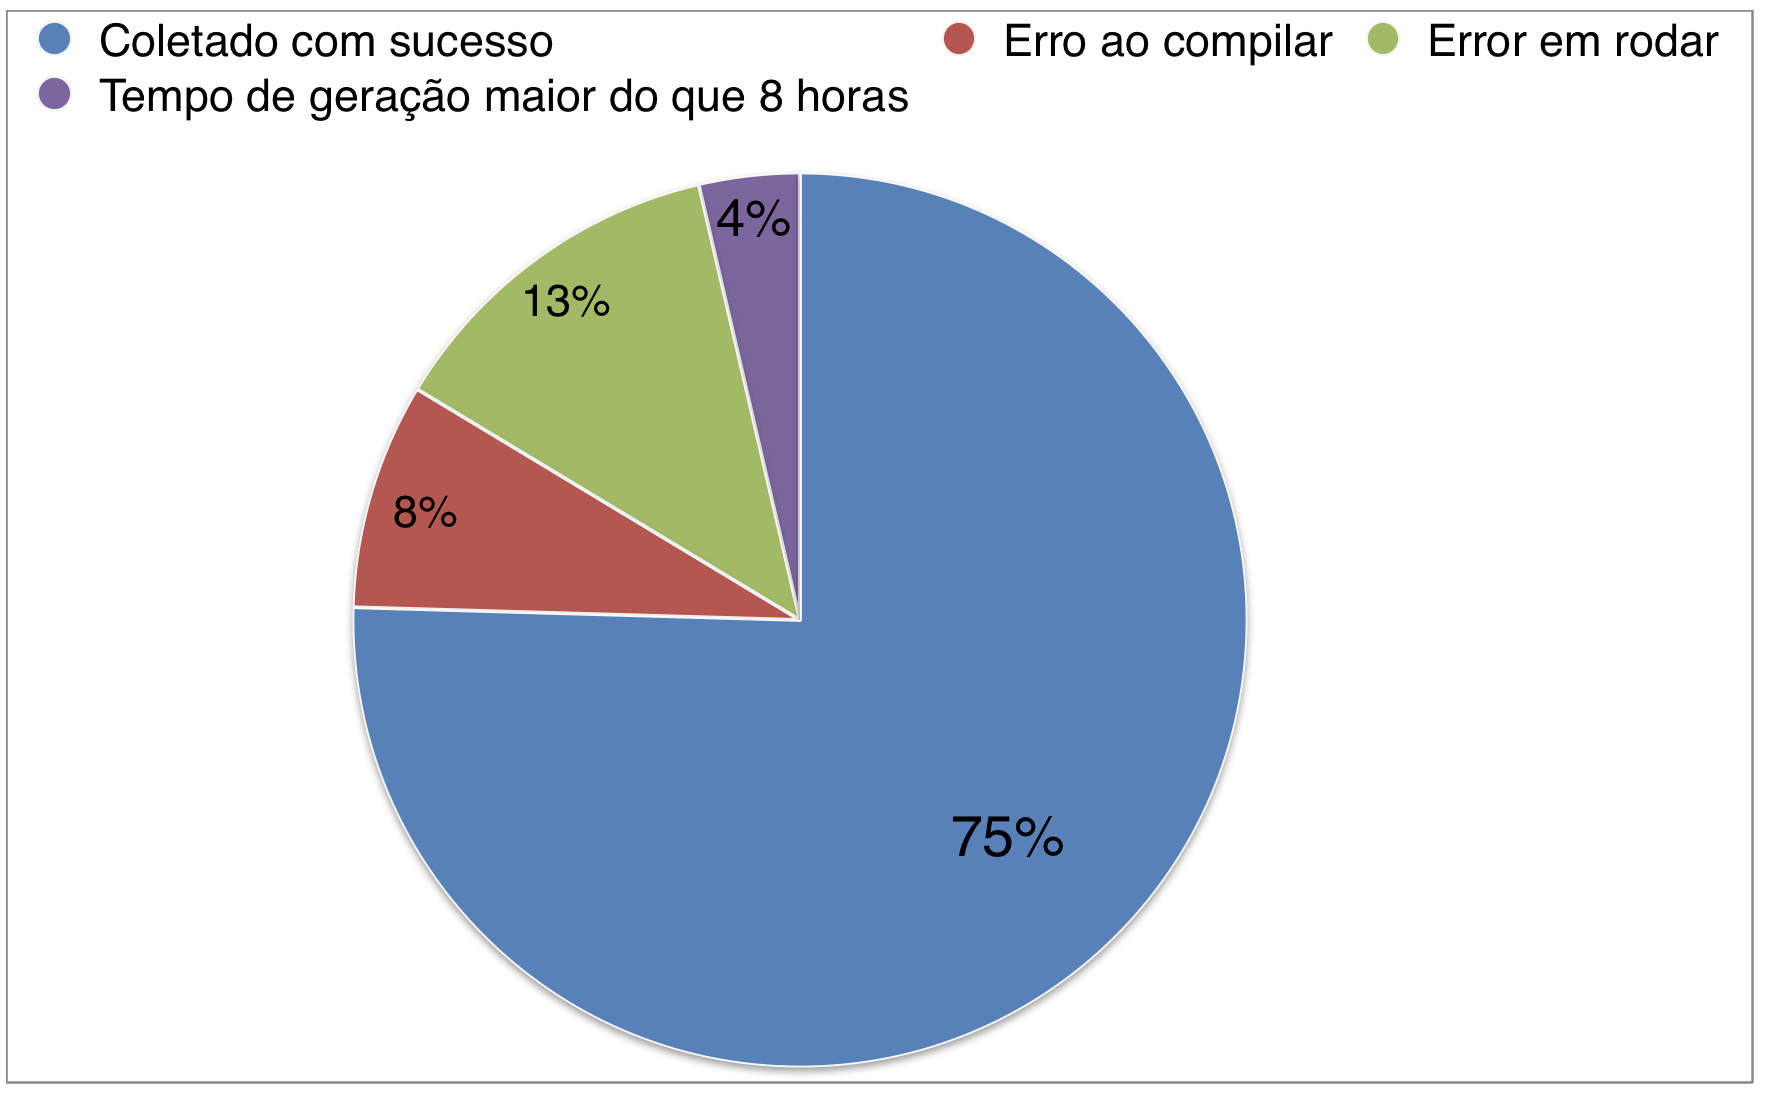
\includegraphics[width=\textwidth]{status_projetos.png}
	\label{fig:distribuicao-estados-projetos}
  \source{Gustavo da Mota Ramos, 2018}
\end{figure}

Como demonstrado na figura \ref{fig:distribuicao-estados-projetos}, da quantidade total de projetos presentes no SF110, 75\% tiveram seus dados de teste gerados corretamente, enquanto 8\% apresentaram problemas ao serem compilados, 13\% foram compilados corretamente porém apresentaram erros duranta geração dos dados de teste e 4\% dos projetos precisaram ter sua execução interrompida pois o processo já havia atingido 8 horas de duração para um único projeto.

Seguido à geração de dados de teste por meio de algoritmos genéticos, a geração de dados de teste por meio da técnica randômica ocorreu, porém esta ocorreu somente nos projetos com sucesso na geração anterior, isso ocorre por conta da comparação ser entre os dois algoritmos, então é necessário que ambos sejam gerados com base nos mesmos projetos.

\begin{figure}[H]% H manda colocar exatamente nessa posição no texto (relativa aos parágrafos anterior e posterior)
	\centering
 	  \caption{Quantidade de classes que atingiram cobertura de código superior ao outro algoritmo}
		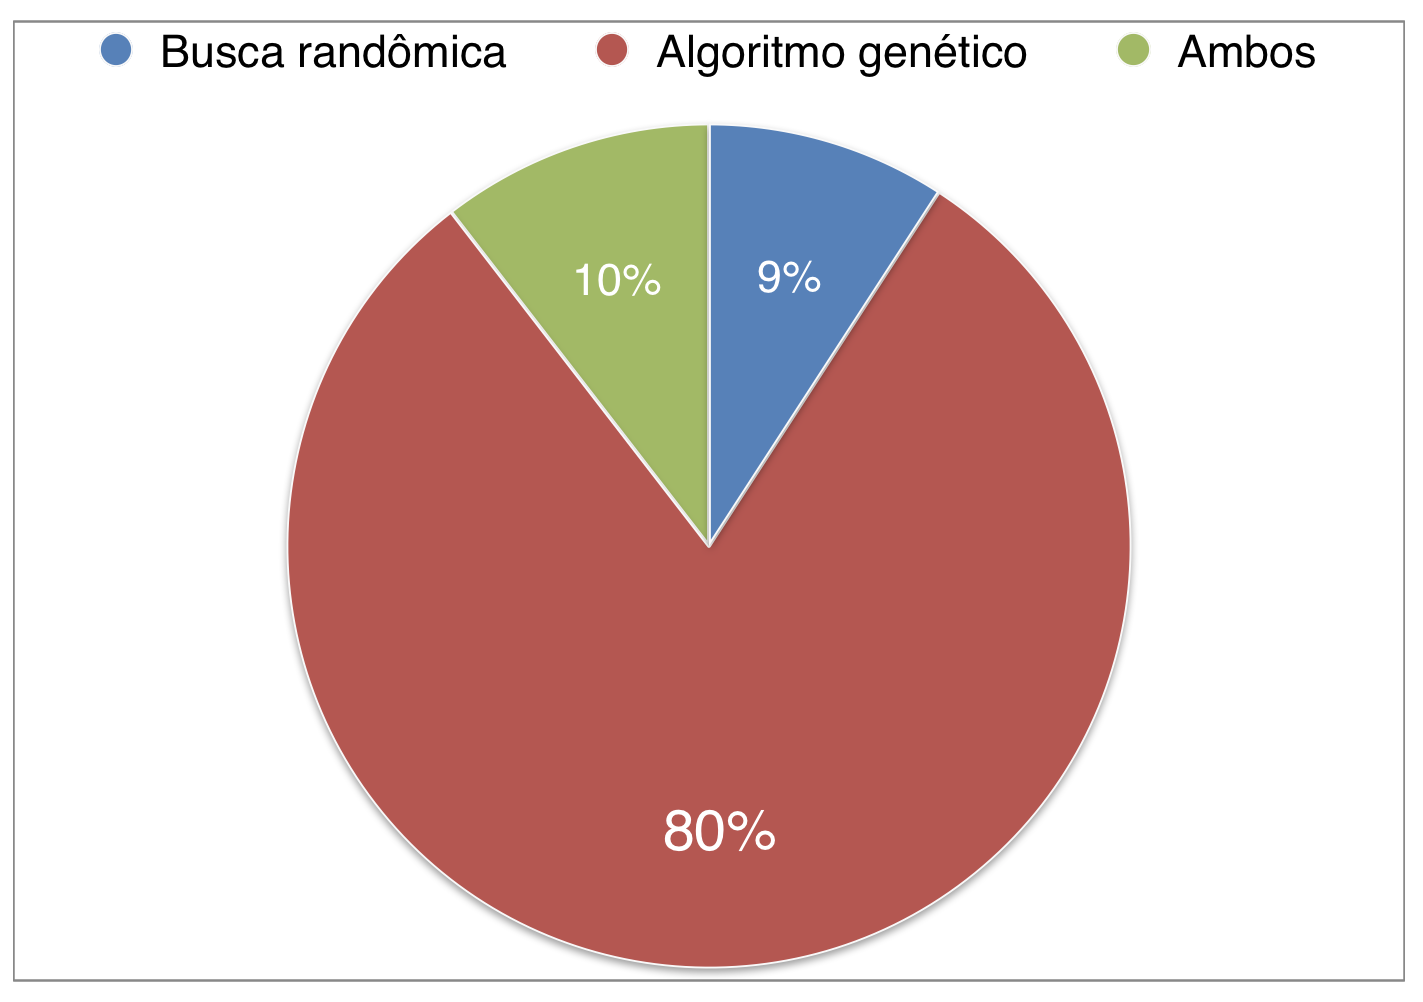
\includegraphics[width=\textwidth]{cobertura_evosuite.png}
	\label{fig:distribuicao-cobertura-evosuite}
  \source{Gustavo da Mota Ramos, 2018}
\end{figure}

Após a coleta, o dataset contém a cobertura de código atingida até o tempo máximo registrado para cada classe em cada um dos algoritmos de geração descritos no capítulo \autoref{chap:geracao-automatica-dados-teste}, sendo assim foi possível verificar em qual dos algoritmos cada classe teve maior cobertura e quantificar, como demonstrado na figura \ref{fig:distribuicao-cobertura-evosuite}. 

Os resultados de cobertura de código obtidos divergem de alguns resultados apresentados por \cite{shamriski20151115}, no experimento que consistiu em gerar os casos de testes a partir de 1000 classes randomicamente escolhidas do corpus SF110. O estudo em questão apontou que seus resultados sugerem que na prática existe pouca diferença quando os resultados de geração de casos de teste são comparados, concluindo que algoritmos randômicos tenham o mesmo nível de efetividade.

Esta diferença pode ser dada por dois fatores como volume de dados analisado e a evolução da ferramenta, o estudo citado utilizou em torno de de 20\% das classes utilizadas para análise na figura \ref{fig:distribuicao-cobertura-evosuite}, o volume maior análisado pode representar uma quantidade maior de casos. Outro fator importante é a evolução da ferramenta EvoSuite ao longo de 3 anos anos, que através de melhorias constantes pode ter causado melhorias no algoritmo genético o suficiente para conseguir o aumento da cobertura de código demonstrado na diferença dos experimentos.

A partir dos dados de cobertura coletados em cada algoritmo, foi possível calcular a diferença entre eles em cada classe. As diferenças foram agrupadas e separadas em diferentes faixas como demonstrado na tabela a seguir:



\begin{table}[h]

\centering
\caption{Distruibuição das classes nas diferenças de cobertura entre os algoritmos}
\vspace{0.5cm}
\begin{tabular}{r|lr}

DIferença de cobertura & Quantidade de classes \\ % Note a separação de col. e a quebra de linhas
\hline                               % para uma linha horizontal
Sem diferença  & 	585 \\
10\%	& 	4232 \\
20\%	& 	1075 \\
30\%	& 	197 \\
40\%	& 	74 \\
50\%	& 	22 \\
60\%	& 	1 \\
70\%	& 	3 \\
80\%	& 	0 \\
90\%	& 	0 \\
100\%	& 	2


\end{tabular}
\label{table:distribuicao-diferenca-cobertura-porcentagem}
\end{table}

O conteúdo da tabela \ref{table:distribuicao-diferenca-cobertura-porcentagem} mostra a distruibuição das diferenças de cobertura, é possível notar que maioria das classes, 85.7 \% do total, possuem diferença de cobertura entre os algoritmos maior do que 0\% e  menor do que 20\%. A diferença de cobertura entre 0\% e 10\% pode ser melhor vista na imagem \ref{fig:grafico_dif_cobertura}. 

\begin{figure}[H]% H manda colocar exatamente nessa posição no texto (relativa aos parágrafos anterior e posterior)
	\centering
 	  \caption{Quantidade de classes que consumiram menos tempo melhor em cada algoritmo}
		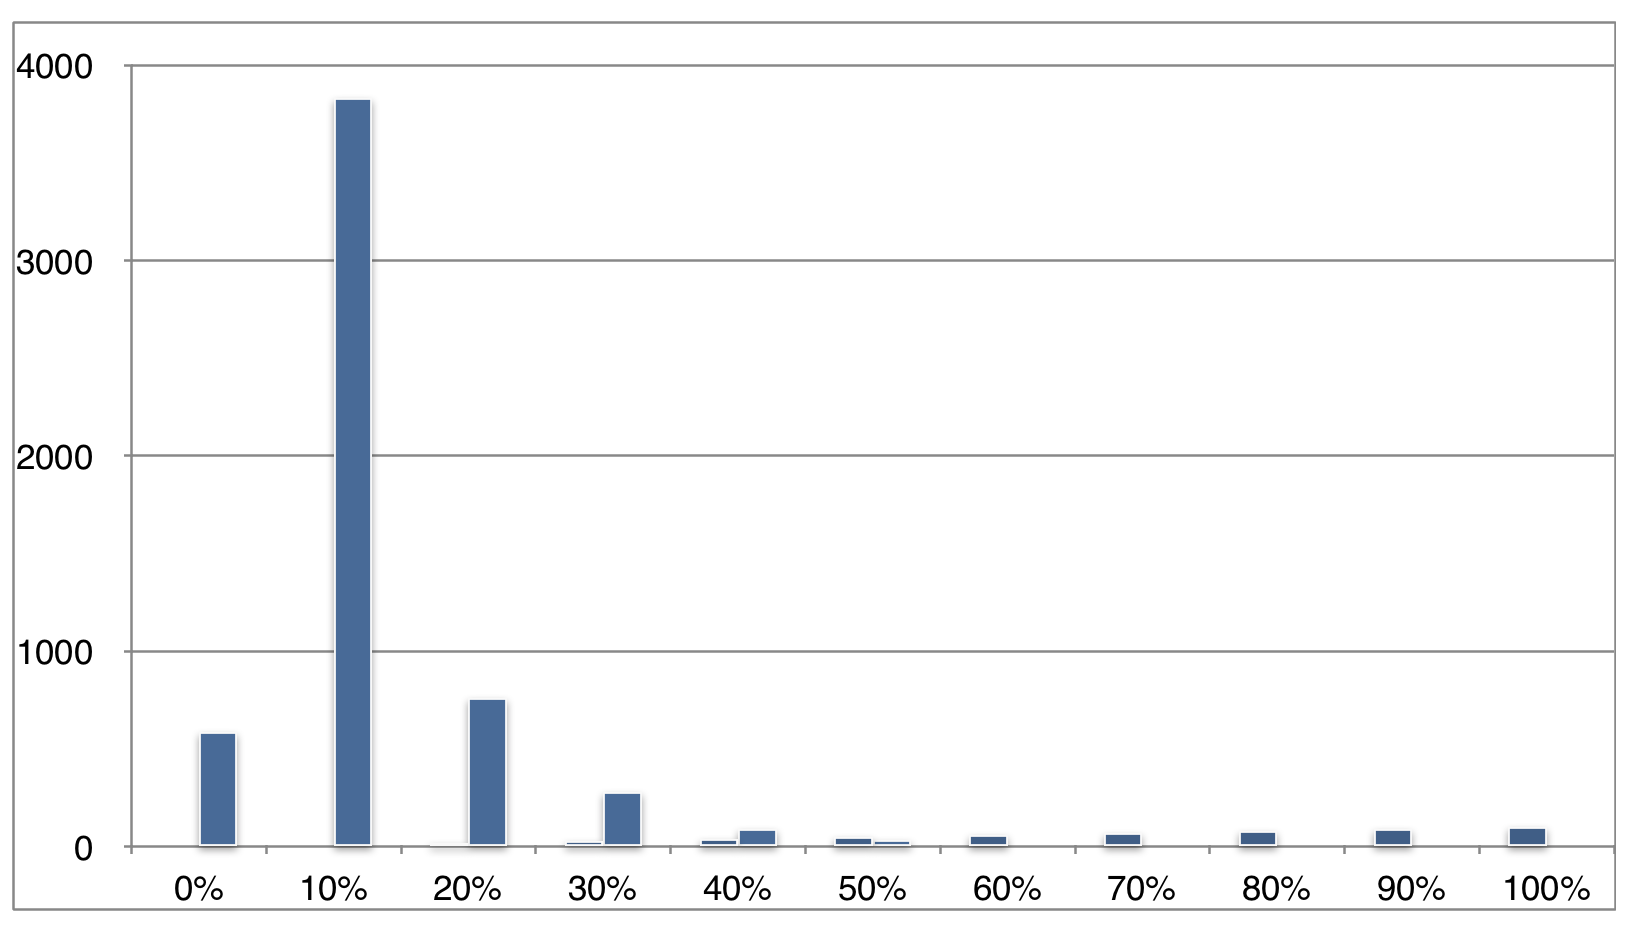
\includegraphics[width=\textwidth]{grafico_dif_cobertura.png}
	\label{fig:grafico_dif_cobertura}
  \source{Gustavo da Mota Ramos, 2018}
\end{figure}


A partir da imagem \ref{fig:grafico_dif_cobertura} é possível notar que a predominância da diferença de cobertura entre as técnicas situa-se entre 0\% e 10\% . Estes valores são importantes para compreender a magniture da diferença coberta entre os algoritmos para que assim seja possível escolher o algoritmo mais rápido em casos que a diferença seja menor ao construir o conjunto de dados de aprendizado.

Um segundo ponto importante de análise é o tempo de geração utilizado em cada um dos algoritmos, em alguns dos projetos análisados, o tempo de geração total foi superior a 8 horas. o mesmo processo aplicado para análise da cobertura do código foi aplicado para o tempo de geração:\\

\begin{figure}[H]% H manda colocar exatamente nessa posição no texto (relativa aos parágrafos anterior e posterior)
	\centering
 	  \caption{Quantidade de classes que consumiram menos tempo melhor em cada algoritmo}
		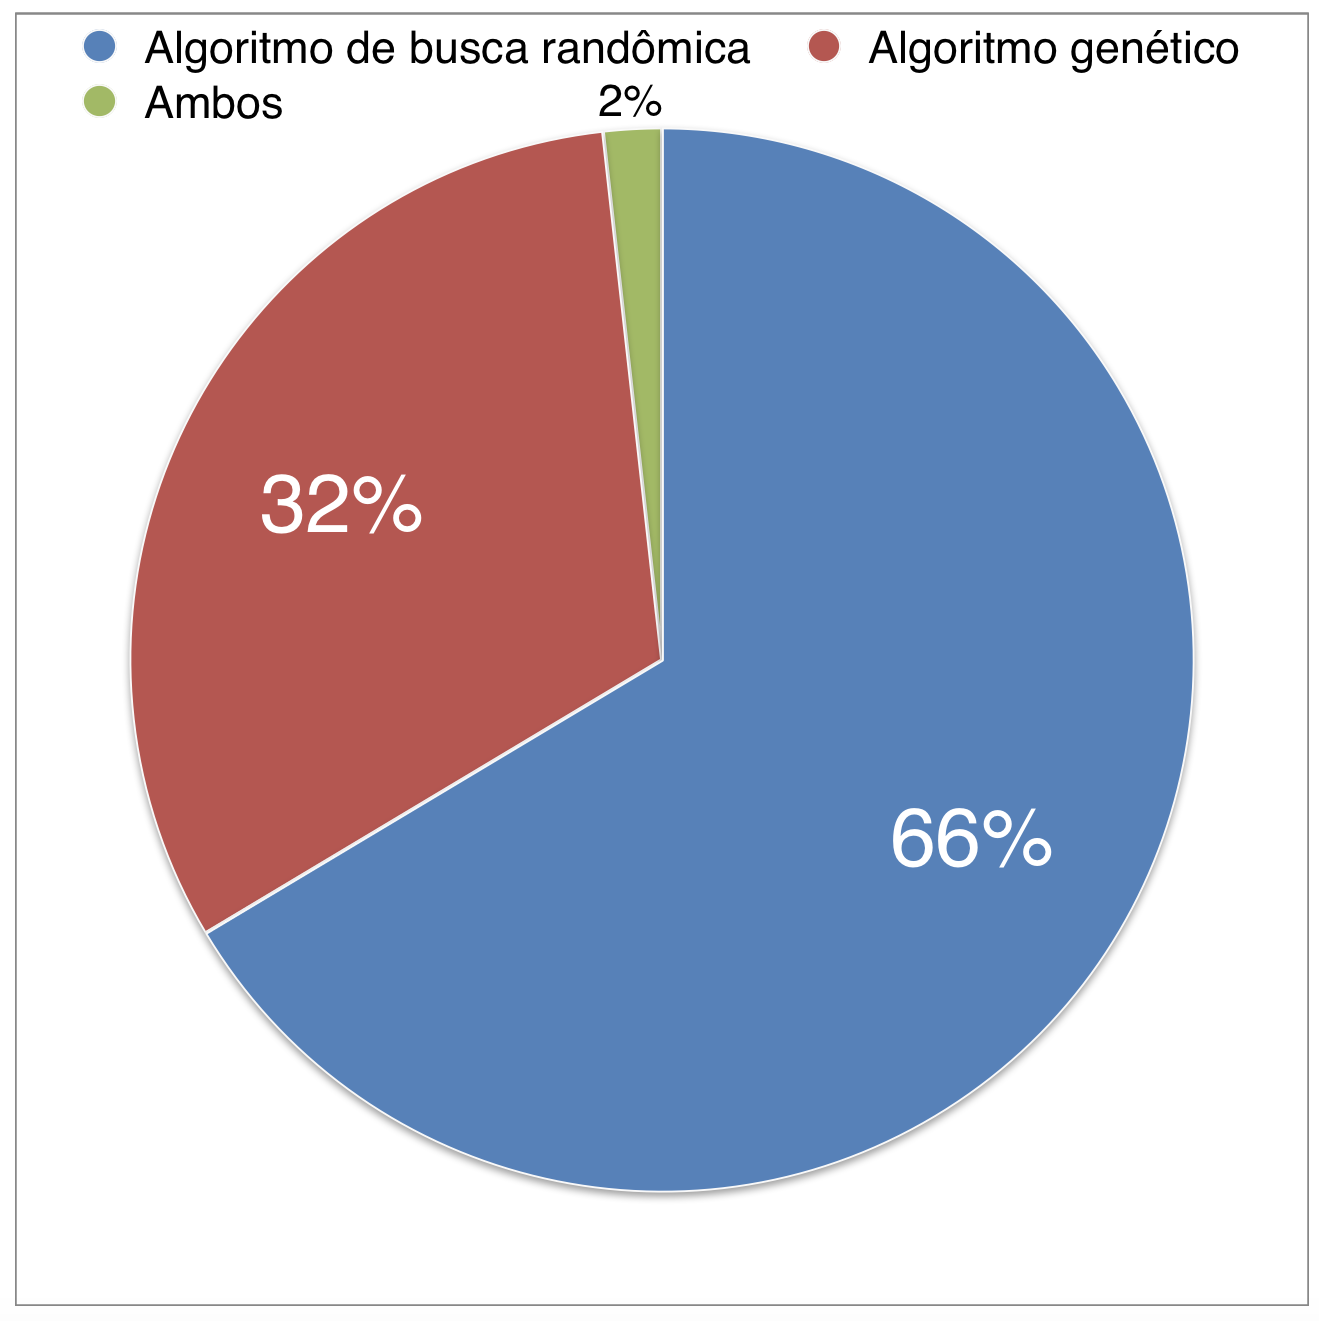
\includegraphics[width=\textwidth]{tempo_evosuite.png}
	\label{fig:distribuicao-tempo-evosuite}
  \source{Gustavo da Mota Ramos, 2018}
\end{figure}

Como pode ser visto na imagem \ref{fig:distribuicao-tempo-evosuite}, uma quantidade considerável, totalizando 66\% das classes foram geradas mais rapidamente utilizando o algoritmo de busca randômica, enquanto somente 32\% das classes tiveram seus dados gerados mais rapidamente utilizando algoritmo genético e somente 2\% tiveram seus dados gerados com a mesma quantidade de tempo.

Após a extração das métricas CK os dados foram consolidados por meio de executáveis escritos em Go, os arquivos de entrada consistem nos resultados gerados usando algoritmo genético, resultados gerados usando algoritmo randômico e as métricas CK. Os 3 arquivos diferem em suas estruturas, porém foram consolidados por meio de umconjunto de dados em comum pelos 3 arquivos: Todos possuem o caminho completo do pacote onde a classe encontra-se e o nome da classe, formando uma tupla única de união das três fontes de dados; O resultado final consistiu em um dataset de 5705 registros de classes contendo os dados consolidados, resultando assim no cálculo da correlação:


\begin{table}[h]
\centering
\caption{Correlação entre métricas CK e cobertura de código}
\vspace{0.5cm}
\begin{tabular}{r|lr}

										
Métrica & Algoritmo genético & Algoritmo randômico \\ % Note a separação de col. e a quebra de linhas
\hline                               % para uma linha horizontal
CBO	& -0.249850668595503	& 	-0.232931214471127 \\
WMC	& -0.29807261754159	& 	-0.276826266943643 \\
DIT	& -0.221073021178272		& -0.229483879955976 \\
NOC& 	0.000302617656848	& 	0.001561246261131 \\
RFC	& -0.564049275058188		& -0.552823956941685 \\
LCOM	 & -0.040802466405277	& 	-0.032051943296475 \\
NOM	& -0.109889786736834		& -0.0827808149062 \\
NOPM	 & -0.014135793315715		& 0.009596758553157 \\
NOSM	 & -0.075230386707179	& 	-0.071445190069526 \\
NOF	& -0.140224056429869	& 	-0.120339077987188 \\
NOPF	& -0.004633572435886		& -0.000497241219225 \\
NOSF	& -0.111343334357608		& -0.109334015568744 \\
NOSI	& -0.282084913928777	& 	-0.273109674212372 \\
LOC	& -0.287212833651501	& 	-0.262779424522538

\end{tabular}
\source{Gustavo Ramos, 2018}
\label{table:correlacao-cobertura}
\end{table}


\begin{table}[h]
\centering
\caption{Correlação entre métricas CK e o tempo de geração}
\vspace{0.5cm}
\begin{tabular}{r|lr}

										
Métrica & Algoritmo genético & Algoritmo randômico \\ % Note a separação de col. e a quebra de linhas
\hline                               % para uma linha horizontal
CBO		& 0.396318591856812		& 0.037898357322244 \\
WMC		& 0.484002414944669		& 0.059460693763974 \\
DIT		& 0.0040537265288		& 0.005185276134757 \\
NOC		& 0.008046221302802		& -0.00048066394787 \\
RFC		& 0.491425142687552		& 0.073355181869394 \\
LCOM		& 0.186475399697658	& 	0.025181662291855 \\
NOM		& 0.441803537967141		& 0.038466136152881 \\
NOPM		& 0.38853663183873		& 0.027876177461111 \\
NOSM		& 0.180912744473895	& 	0.030067038091283 \\
NOF		& 0.332907657997746	& 	0.02963776551629 \\
NOPF		& 0.059216533461886	& 	0.002387027385852 \\
NOSF		& 0.159268739166119		& 0.02786927036709 \\
NOSI		& 0.283074420386565		& 0.042066832430523 \\
LOC		& 0.476423297500777	& 0.052316363027409
\end{tabular}
\source{Gustavo Ramos, 2018}
\label{table:correlacao-tempo}
\end{table}

As tabelas \ref{table:correlacao-cobertura} e \ref{table:correlacao-tempo} possuem as correlações calculadas entre cada métrica $CK$ extraída com a cobertura atingida nos dois algoritmos. A partir dos resultados presentes nas tabelas é possível notar que os valores de correlação situados entre valores baixos e moderados, enquanto no algoritmo randômico, com exceção da métrica $RFC$, todos os valores baixos o suficiente para não possuírem qualquer significância para análise.

\section{Aplicação das classes e classificação}

Após a coleta dos dados e consolidação seguido de validação deste conjunto por meio da sua correlação, é possível trabalhar com este conjunto para assim classificar cada um dos elementos. Para a execução de um algoritmo de classificação supervisionado, neste caso o algoritmo naive bayes, é necessário primariamente definir quais são as classes as quais cada elemento do conjunto de dados poderá pertencer, as classes são os nomes dados para os agrupamentos os quais será necessário classificar cada elemento de acordo com suas características, desde que um elemento pertença a uma classe somente.

Dado que o intuito do experimento é reconhecer qual o algoritmo de geração de dados de teste é mais adequado: Algoritmo de busca randômica ou algoritmo genético, é possível então afirmar que as classes de classificação serão os dois algoritmos, os quais serão tratados com as seguintes classes:  \textbf{RANDOM} ou \textbf{GA} respectivamente. 

\subsection{Conjunto de aprendizado com base em cobertura}

O primeiro conjunto de aprendizado montado, levou em consideração somente a cobertura dos testes para montagem do conjunto de aprendizado, ou seja, o tempo foi desconsiderado, sendo assim este conjunto de dados foi nomeado como \textbf{CBCK} (Cover based on CK dataset).

\begin{algorithm}[htbp]
\caption{Algoritmo para aplicação das classes no conjunto de treinamento CBCK}
\label{alg:algoritmo-CBCK}
\begin{algorithmic}[1]

\Procedure{AplicarClasse}{}
\State Para todas as linhas L do conjunto consolidado:
\State $classe := RANDOM$
\State 		Se L.CoberturaGA > L.CoberturaRandom: $classe := GA$
\State $AtualizaArquivo()$
\EndProcedure
\end{algorithmic}
\source{Gustavo Ramos, 2018}
\end{algorithm}

O algoritmo \ref{alg:algoritmo-CBCK} demonstra a lógica para aplicação da classe para cada linha do conjunto de testes como é possível ver na linha 2. A partir da linha 3 é possível ver que todas as linhas receberam a classe \textbf{RANDOM} , este estado é mudado se a condição da linha 4 seja for satisfeita, ou seja, a linha do conjunto receberá a  \textbf{GA} se a cobertura com algoritmo genético for maior. A atribuição da linha 3 ocorreu pois além dos casos em que o algoritmo ranômico tenha maior performance, é possível ocorrer o caso em que ambas ambas cobriram a mesma quantidade, estes são os 10\% presentes na figura \ref{fig:distribuicao-cobertura-evosuite}. Para os casos em que a cobertura atingida foi igual nos dois algoritmos, a classe  \textbf{RANDOM}  foi aplicada visto que esta consumiu menor tempo na geração de dados como demonstrado na figura \ref{fig:distribuicao-tempo-evosuite}.

Após a aplicação das classes no conjunto de dados, é possível utilizar o mesmo na ferramenta Weka para assim executar o algoritmo de classificação naive bayes, a própria ferramenta possui um mecanismo onde é possível separar aleatoriamente uma quantidade dos dados do conjunto para treinamento e a parte complementar (usualmente menor) para validação e testes, por padrão foi adotado 80\% dos dados para aprendizado enquanto os 20\% restantes para testes. O algoritmo foi executado apresentando dois resultados, a precisão e a seguinte matriz de confusão:

\begin{table}[h]
\centering
\caption{Matriz de confusão ao classificar o conjunto CBCK com o algoritmo Naive Bayes}
\vspace{0.5cm}
\begin{tabular}{r|lr}

										
 & GA & RANDOM \\ % Note a separação de col. e a quebra de linhas
\hline                               % para uma linha horizontal
GA		& 898		& 42 \\
RANDOM		& 176		& 25
\end{tabular}
\source{Gustavo Ramos, 2018}
\label{table:confusao-CBCK}
\end{table}

Os resultados apresentados pela ferramenta demonstram que 78.6\% dos casos foram corretamente classificados enquanto 21.4\% foram incorretamente classificados. A matriz demonstrada na tabela \ref{table:confusao-CBCK} é chamada de matriz de confusão, as coordenadas na diagonal (Os valores 898 e 25 respectivamente) representam os casos corretamente classificados, ou seja, a linha possuía a classe GA no conjunto de treinamento e foi corretamente classificada como GA, o mesmo casso ocorre para a classe RANDOM. Os outros casos compõe os casos onde uma classe foi dada e o algoritmo classificou em outra classe.

É possível notar, apesar da precisão de 78.6\%, que o algoritmo teve maior facilidade de classificar casos onde o algoritmo genético possuiu maior cobertura, porém possui dificuldade em classificar em torno de 60\% dos casos onde o algoritmo randômico possuiu atingiu maior cobertura.

No conjunto de aprendizado \textbf{CBCK}, 14 métricas de softwares orientados a objetos foram utilizadas, como as métricas listadas nas tabelas  \ref{table:correlacao-cobertura} e \ref{table:correlacao-tempo}, porém \cite{Xia2013} afirma que algumas métricas tornam-se redundantes ou irrelevantes em um modelo relacionado à predição de defeitos em softwares.

Os resultados simulados por \cite{Xia2013} provam que diversas métricas são correlacionadas e algumas podem ser úteis em modelos de predição de defeitos, métricas destritas no capitulo \ref{chap:metricas}  como: LOC, RFC, CBO, AMC e CAM.  As métricas destacadas coincidem inclusive com as de valores mais altos de correlação na tabela \ref{table:correlacao-cobertura}.

Dada a relevâncias das métricas citadas, segundo conjunto de aprendizado foi criado com o nome \textbf{CBCK+} com base no conjunto de métricas detalhados por \cite{Xia2013}, ou seja, somente estas métricas foram selecionadas para execução do algorítmo na interface do software Weka. Dado que as métricas de coesão entre os métodos (CAM) e complexidade média dos métodos não fazem parte do conjunto, estas foram substituídas pelas métricas LCOM e WMC respectivamente, resultando na seguinte matriz de confusão:

\begin{table}[h]
\centering
\caption{Matriz de confusão ao classificar o conjunto CBCK com o algoritmo Naive Bayes}
\vspace{0.5cm}
\begin{tabular}{r|lr}

										
 & GA & RANDOM \\ % Note a separação de col. e a quebra de linhas
\hline                               % para uma linha horizontal
GA		& 891		& 49 \\
RANDOM		& 176		& 25
\end{tabular}
\source{Gustavo Ramos, 2018}
\label{table:confusao-CBCK+}
\end{table}

O algoritmo naive bayes, ao ser executado, retornou uma precisão de 80.3\% após a otimização, a partir da matriz de confusão \ref{table:confusao-CBCK+} é possível notar que a classificação de algoritmos randômicos possuiu uma melhora modesta de 1.7\%. 

\subsection{Conjunto de aprendizado híbrido}

O terceiro conjunto de aprendizado construído levou em consideração tanto a cobertura dos testes quanto o tempo de execução, a execução do algoritmo foi similar ao algoritmo \ref{alg:algoritmo-CBCK} com uma otimização: Em casos onde a diferença de cobertura entre os algoritmos situa-se entre 0\% e 10\%, a classe do algoritmo com o menor tempo de execução foi aplicada, o conjunto de treinamento foi então nomeado por \textbf{CBCK10}. O algoritmo naive bayes foi executado, seguindo o uso das mesmas métricas utilizadas no conjunto de treinamento \textbf{CBCK+}, resultando na seguinte matriz de confusão:

\begin{table}[h]
\centering
\caption{Matriz de confusão ao classificar o conjunto CBCK10 com o algoritmo Naive Bayes}
\vspace{0.5cm}
\begin{tabular}{r|lr}

										
 & GA & RANDOM \\ % Note a separação de col. e a quebra de linhas
\hline                               % para uma linha horizontal
GA		& 524		& 284 \\
RANDOM		& 107		& 226
\end{tabular}
\source{Gustavo Ramos, 2018}
\label{table:confusao-hibrido-plus}
\end{table}

O algoritmo, ao ser executado, retornou uma precisão de 63.5\%, porém é possível notar a melhora na distribuição da matriz de confusão demonstrada na tabela \ref{table:confusao-hibrido-plus}, o algoritmo passou a reconhecer mais casos onde o algoritmo randômico deveria ser selecionado enquanto o algoritmo reconheceu uma grande quantidade dos casos onde o algoritmo genético deveria ser selecionado.




\chapter{Conclusão}
\label{chap:conclusao}
Neste trabalho foi apresentado um estudo sobre a relação das métricas CK com a cobertura de código e tempo em dois algoritmos de geração de dados de testes distintos.
Ao longo do trabalho foram coletados diversos dados sobre ambos os assuntos: métricas e geração de dados de testes, estes dados foram então processados, agrupados e análisados para que assim seja compreendida a relação entre estes, caso exista e possíveis tomadas de decisão.

Nas etapas iniciais de projeto, algumas questões foram levantadas como as questões elicitadas no capítulo \ref{chap:introducao}, estas questões serviram como base para mapear todos os materiais e atividades necessários para garantir respostas. Após as  extrações e análises  descritas no capítulo \ref{chap:resultados}, é possível assim responder os questionamentos, dentro os questionamentos estão:\\

\fbox{\parbox{5in}{%
Q1: Existe alguma diferença de performance entre os algoritmos de geração de dados de teste: randômico e algoritmos genéticos ?
}}
\\

Os algoritmos apresentados possuem diferenças em seus resultados de execução, sejam eles cobertura de código ou tempo de execução. O algoritmo genético apresentou maior porcentagem de cobertura de código em 80\% dos casos analisados, estas diferenças situam-se em sua maioria entre 1\% e 20\% quando comparados às coberturas de código apresentadas pelo algoritmo randômico nos testes efetuados. Esta diferença pode ser dada por conta da natureza do algoritmo genético, este é um algoritmo de busca direcionado o qual altera sua própria execução para o problema de busca em análise, enquanto o algoritmo randômico procura possíveis soluções em um espaço maior de busca, com pouco direcionamento.

Em comparação, o algoritmo randômico apresentou menor tempo de execução em 66 \% dos casos, o tempo de execução reduzido é dado pelo tempo entre as interações do algoritmo, visto que o algoritmo randômico não possui passos como crossover ou mutação, garantindo assim que consiga varrer o espaço de busca com velocidade maior se comparado ao algoritmo genético.

Sendo assim, é possível concluir que o algorítmo randômico consegue ser executado com maior velocidade e menor tempo do que um algoritmo genético, porém também é notável que um algorítmo genético consegue atingir maior cobertura de código.\\

\fbox{\parbox{5in}{%
Q2: Alguma característica ou conjunto de características do software sob teste que faça com que uma técnica usada na geração de casos de teste seja melhor do que outra?
}}
\\

Em suma, 14 métricas foram analisadas no contexto de geração de dados de teste para entender características como correlação com o tempo necessário para geração ou a cobertura de código atingida ou efeitos destas métricas no processo de geração. Durante a análise dos resultados foi possível notar que um número maior de métricas pode ser redundante, inclusive danificar o resultado se comparado a um conjunto mais preciso de métricas.

Através a análise foi possível notar também que um conjunto de 5 métricas foram capazes de representar melhor uma classe durante a seleção de algoritmos quando este conjunto foi comparado ao conjunto total de 14 métricas. Neste conjunto de métricas estão: $CBO$ (Coupling between Object Classes), $WMC$ (Weight Method Class ou Complexidade de McCabe), $LCOM$ (Lack of Cohesion of Methods) e $LOC$ (Lines of code) e em especial a métrica $RFC$ (Response for a Class) a qual possuiu maior valor de correlação com a cobertura de código.

O conjunto das 5 métricas citadas apresentou correlação média com a cobertura de código apresentada pelo algoritmo genético, além de demonstrar eficiência no algoritmo de classificação, ao mesmo tempo,  as métricas apresentaram pouca correlação com a cobertura obtida pelo algoritmo randômico ou com o tempo de execução em ambos os algoritmos, sendo assim, é possível afirmar que um algorítmo genético tem características similares em geração de dados de teste enquanto este fato não ocorre no algoritmo randômico. \\


\fbox{\parbox{5in}{%
Q3: É possível escolher entre dois algoritmos de geração de dados de testes a partir de um algoritmo de classificação e métricas de softwares orientados e objetos ?
}}
\\





% ----------------------------------------------------------
% ELEMENTOS PÓS-TEXTUAIS
% ----------------------------------------------------------
\postextual
% ----------------------------------------------------------

% ----------------------------------------------------------
% Referências bibliográficas
% ----------------------------------------------------------
\bibliography{referencias}

% ----------------------------------------------------------
% Glossário
% ----------------------------------------------------------
%
% Consulte o manual da classe abntex2 para orientações sobre o glossário.
%
%\glossary

% ----------------------------------------------------------
% Apêndices
% ----------------------------------------------------------

% ---
% Inicia os apêndices
% ---
\begin{apendicesenv}

% Imprime uma página indicando o início dos apêndices
%\partapendices

%-------------------------------------------------------------------------
% Comentário adicional do PPgSI - Informações sobre ``apêndice''
%
% Para todos os captions/(títulos) (de seções, subseções, tabelas, 
% ilustrações, etc.):
%     - em maiúscula apenas a primeira letra da sentença (do título), 
%       exceto nomes próprios, geográficos, institucionais ou Programas ou
%       Projetos ou siglas, os quais podem ter letras em maiúscula também.
%
% Todas  as tabelas, ilustrações (figuras, quadros, gráficos etc. ), 
% anexos, apêndices devem obrigatoriamente ser citados no texto.
%      - a citação deve vir sempre antes da primeira vez em que a tabela, 
%        ilustração etc., aparecer pela primeira vez.
%
%-------------------------------------------------------------------------




\end{apendicesenv}
% ---


% ----------------------------------------------------------
% Anexos
% ----------------------------------------------------------

% ---
% Inicia os anexos
% ---
\begin{anexosenv}

% Imprime uma página indicando o início dos anexos
%\partanexos


%-------------------------------------------------------------------------
% Comentário adicional do PPgSI - Informações sobre ``anexo''
%
% Para todos os captions/(títulos) (de seções, subseções, tabelas, 
% ilustrações, etc.):
%     - em maiúscula apenas a primeira letra da sentença (do título), 
%       exceto nomes próprios, geográficos, institucionais ou Programas ou
%       Projetos ou siglas, os quais podem ter letras em maiúscula também.
%
% Todas  as tabelas, ilustrações (figuras, quadros, gráficos etc. ), 
% anexos, apêndices devem obrigatoriamente ser citados no texto.
%      - a citação deve vir sempre antes da primeira vez em que a tabela, 
%        ilustração etc., aparecer pela primeira vez.
%
%-------------------------------------------------------------------------


\end{anexosenv}

%---------------------------------------------------------------------
% INDICE REMISSIVO
%---------------------------------------------------------------------
%%%%%MF\phantompart
%%%%%MF\printindex
%---------------------------------------------------------------------

\end{document}
